% Options for packages loaded elsewhere
\PassOptionsToPackage{unicode}{hyperref}
\PassOptionsToPackage{hyphens}{url}
\PassOptionsToPackage{dvipsnames,svgnames,x11names}{xcolor}
%
\documentclass[
  letterpaper,
  DIV=11,
  numbers=noendperiod]{scrartcl}

\usepackage{amsmath,amssymb}
\usepackage{iftex}
\ifPDFTeX
  \usepackage[T1]{fontenc}
  \usepackage[utf8]{inputenc}
  \usepackage{textcomp} % provide euro and other symbols
\else % if luatex or xetex
  \usepackage{unicode-math}
  \defaultfontfeatures{Scale=MatchLowercase}
  \defaultfontfeatures[\rmfamily]{Ligatures=TeX,Scale=1}
\fi
\usepackage{lmodern}
\ifPDFTeX\else  
    % xetex/luatex font selection
\fi
% Use upquote if available, for straight quotes in verbatim environments
\IfFileExists{upquote.sty}{\usepackage{upquote}}{}
\IfFileExists{microtype.sty}{% use microtype if available
  \usepackage[]{microtype}
  \UseMicrotypeSet[protrusion]{basicmath} % disable protrusion for tt fonts
}{}
\makeatletter
\@ifundefined{KOMAClassName}{% if non-KOMA class
  \IfFileExists{parskip.sty}{%
    \usepackage{parskip}
  }{% else
    \setlength{\parindent}{0pt}
    \setlength{\parskip}{6pt plus 2pt minus 1pt}}
}{% if KOMA class
  \KOMAoptions{parskip=half}}
\makeatother
\usepackage{xcolor}
\setlength{\emergencystretch}{3em} % prevent overfull lines
\setcounter{secnumdepth}{-\maxdimen} % remove section numbering
% Make \paragraph and \subparagraph free-standing
\makeatletter
\ifx\paragraph\undefined\else
  \let\oldparagraph\paragraph
  \renewcommand{\paragraph}{
    \@ifstar
      \xxxParagraphStar
      \xxxParagraphNoStar
  }
  \newcommand{\xxxParagraphStar}[1]{\oldparagraph*{#1}\mbox{}}
  \newcommand{\xxxParagraphNoStar}[1]{\oldparagraph{#1}\mbox{}}
\fi
\ifx\subparagraph\undefined\else
  \let\oldsubparagraph\subparagraph
  \renewcommand{\subparagraph}{
    \@ifstar
      \xxxSubParagraphStar
      \xxxSubParagraphNoStar
  }
  \newcommand{\xxxSubParagraphStar}[1]{\oldsubparagraph*{#1}\mbox{}}
  \newcommand{\xxxSubParagraphNoStar}[1]{\oldsubparagraph{#1}\mbox{}}
\fi
\makeatother

\usepackage{color}
\usepackage{fancyvrb}
\newcommand{\VerbBar}{|}
\newcommand{\VERB}{\Verb[commandchars=\\\{\}]}
\DefineVerbatimEnvironment{Highlighting}{Verbatim}{commandchars=\\\{\}}
% Add ',fontsize=\small' for more characters per line
\usepackage{framed}
\definecolor{shadecolor}{RGB}{241,243,245}
\newenvironment{Shaded}{\begin{snugshade}}{\end{snugshade}}
\newcommand{\AlertTok}[1]{\textcolor[rgb]{0.68,0.00,0.00}{#1}}
\newcommand{\AnnotationTok}[1]{\textcolor[rgb]{0.37,0.37,0.37}{#1}}
\newcommand{\AttributeTok}[1]{\textcolor[rgb]{0.40,0.45,0.13}{#1}}
\newcommand{\BaseNTok}[1]{\textcolor[rgb]{0.68,0.00,0.00}{#1}}
\newcommand{\BuiltInTok}[1]{\textcolor[rgb]{0.00,0.23,0.31}{#1}}
\newcommand{\CharTok}[1]{\textcolor[rgb]{0.13,0.47,0.30}{#1}}
\newcommand{\CommentTok}[1]{\textcolor[rgb]{0.37,0.37,0.37}{#1}}
\newcommand{\CommentVarTok}[1]{\textcolor[rgb]{0.37,0.37,0.37}{\textit{#1}}}
\newcommand{\ConstantTok}[1]{\textcolor[rgb]{0.56,0.35,0.01}{#1}}
\newcommand{\ControlFlowTok}[1]{\textcolor[rgb]{0.00,0.23,0.31}{\textbf{#1}}}
\newcommand{\DataTypeTok}[1]{\textcolor[rgb]{0.68,0.00,0.00}{#1}}
\newcommand{\DecValTok}[1]{\textcolor[rgb]{0.68,0.00,0.00}{#1}}
\newcommand{\DocumentationTok}[1]{\textcolor[rgb]{0.37,0.37,0.37}{\textit{#1}}}
\newcommand{\ErrorTok}[1]{\textcolor[rgb]{0.68,0.00,0.00}{#1}}
\newcommand{\ExtensionTok}[1]{\textcolor[rgb]{0.00,0.23,0.31}{#1}}
\newcommand{\FloatTok}[1]{\textcolor[rgb]{0.68,0.00,0.00}{#1}}
\newcommand{\FunctionTok}[1]{\textcolor[rgb]{0.28,0.35,0.67}{#1}}
\newcommand{\ImportTok}[1]{\textcolor[rgb]{0.00,0.46,0.62}{#1}}
\newcommand{\InformationTok}[1]{\textcolor[rgb]{0.37,0.37,0.37}{#1}}
\newcommand{\KeywordTok}[1]{\textcolor[rgb]{0.00,0.23,0.31}{\textbf{#1}}}
\newcommand{\NormalTok}[1]{\textcolor[rgb]{0.00,0.23,0.31}{#1}}
\newcommand{\OperatorTok}[1]{\textcolor[rgb]{0.37,0.37,0.37}{#1}}
\newcommand{\OtherTok}[1]{\textcolor[rgb]{0.00,0.23,0.31}{#1}}
\newcommand{\PreprocessorTok}[1]{\textcolor[rgb]{0.68,0.00,0.00}{#1}}
\newcommand{\RegionMarkerTok}[1]{\textcolor[rgb]{0.00,0.23,0.31}{#1}}
\newcommand{\SpecialCharTok}[1]{\textcolor[rgb]{0.37,0.37,0.37}{#1}}
\newcommand{\SpecialStringTok}[1]{\textcolor[rgb]{0.13,0.47,0.30}{#1}}
\newcommand{\StringTok}[1]{\textcolor[rgb]{0.13,0.47,0.30}{#1}}
\newcommand{\VariableTok}[1]{\textcolor[rgb]{0.07,0.07,0.07}{#1}}
\newcommand{\VerbatimStringTok}[1]{\textcolor[rgb]{0.13,0.47,0.30}{#1}}
\newcommand{\WarningTok}[1]{\textcolor[rgb]{0.37,0.37,0.37}{\textit{#1}}}

\providecommand{\tightlist}{%
  \setlength{\itemsep}{0pt}\setlength{\parskip}{0pt}}\usepackage{longtable,booktabs,array}
\usepackage{calc} % for calculating minipage widths
% Correct order of tables after \paragraph or \subparagraph
\usepackage{etoolbox}
\makeatletter
\patchcmd\longtable{\par}{\if@noskipsec\mbox{}\fi\par}{}{}
\makeatother
% Allow footnotes in longtable head/foot
\IfFileExists{footnotehyper.sty}{\usepackage{footnotehyper}}{\usepackage{footnote}}
\makesavenoteenv{longtable}
\usepackage{graphicx}
\makeatletter
\def\maxwidth{\ifdim\Gin@nat@width>\linewidth\linewidth\else\Gin@nat@width\fi}
\def\maxheight{\ifdim\Gin@nat@height>\textheight\textheight\else\Gin@nat@height\fi}
\makeatother
% Scale images if necessary, so that they will not overflow the page
% margins by default, and it is still possible to overwrite the defaults
% using explicit options in \includegraphics[width, height, ...]{}
\setkeys{Gin}{width=\maxwidth,height=\maxheight,keepaspectratio}
% Set default figure placement to htbp
\makeatletter
\def\fps@figure{htbp}
\makeatother
% definitions for citeproc citations
\NewDocumentCommand\citeproctext{}{}
\NewDocumentCommand\citeproc{mm}{%
  \begingroup\def\citeproctext{#2}\cite{#1}\endgroup}
\makeatletter
 % allow citations to break across lines
 \let\@cite@ofmt\@firstofone
 % avoid brackets around text for \cite:
 \def\@biblabel#1{}
 \def\@cite#1#2{{#1\if@tempswa , #2\fi}}
\makeatother
\newlength{\cslhangindent}
\setlength{\cslhangindent}{1.5em}
\newlength{\csllabelwidth}
\setlength{\csllabelwidth}{3em}
\newenvironment{CSLReferences}[2] % #1 hanging-indent, #2 entry-spacing
 {\begin{list}{}{%
  \setlength{\itemindent}{0pt}
  \setlength{\leftmargin}{0pt}
  \setlength{\parsep}{0pt}
  % turn on hanging indent if param 1 is 1
  \ifodd #1
   \setlength{\leftmargin}{\cslhangindent}
   \setlength{\itemindent}{-1\cslhangindent}
  \fi
  % set entry spacing
  \setlength{\itemsep}{#2\baselineskip}}}
 {\end{list}}
\usepackage{calc}
\newcommand{\CSLBlock}[1]{\hfill\break\parbox[t]{\linewidth}{\strut\ignorespaces#1\strut}}
\newcommand{\CSLLeftMargin}[1]{\parbox[t]{\csllabelwidth}{\strut#1\strut}}
\newcommand{\CSLRightInline}[1]{\parbox[t]{\linewidth - \csllabelwidth}{\strut#1\strut}}
\newcommand{\CSLIndent}[1]{\hspace{\cslhangindent}#1}

\KOMAoption{captions}{tableheading}
\makeatletter
\@ifpackageloaded{tcolorbox}{}{\usepackage[skins,breakable]{tcolorbox}}
\@ifpackageloaded{fontawesome5}{}{\usepackage{fontawesome5}}
\definecolor{quarto-callout-color}{HTML}{909090}
\definecolor{quarto-callout-note-color}{HTML}{0758E5}
\definecolor{quarto-callout-important-color}{HTML}{CC1914}
\definecolor{quarto-callout-warning-color}{HTML}{EB9113}
\definecolor{quarto-callout-tip-color}{HTML}{00A047}
\definecolor{quarto-callout-caution-color}{HTML}{FC5300}
\definecolor{quarto-callout-color-frame}{HTML}{acacac}
\definecolor{quarto-callout-note-color-frame}{HTML}{4582ec}
\definecolor{quarto-callout-important-color-frame}{HTML}{d9534f}
\definecolor{quarto-callout-warning-color-frame}{HTML}{f0ad4e}
\definecolor{quarto-callout-tip-color-frame}{HTML}{02b875}
\definecolor{quarto-callout-caution-color-frame}{HTML}{fd7e14}
\makeatother
\makeatletter
\@ifpackageloaded{caption}{}{\usepackage{caption}}
\AtBeginDocument{%
\ifdefined\contentsname
  \renewcommand*\contentsname{Table of contents}
\else
  \newcommand\contentsname{Table of contents}
\fi
\ifdefined\listfigurename
  \renewcommand*\listfigurename{List of Figures}
\else
  \newcommand\listfigurename{List of Figures}
\fi
\ifdefined\listtablename
  \renewcommand*\listtablename{List of Tables}
\else
  \newcommand\listtablename{List of Tables}
\fi
\ifdefined\figurename
  \renewcommand*\figurename{Figure}
\else
  \newcommand\figurename{Figure}
\fi
\ifdefined\tablename
  \renewcommand*\tablename{Table}
\else
  \newcommand\tablename{Table}
\fi
}
\@ifpackageloaded{float}{}{\usepackage{float}}
\floatstyle{ruled}
\@ifundefined{c@chapter}{\newfloat{codelisting}{h}{lop}}{\newfloat{codelisting}{h}{lop}[chapter]}
\floatname{codelisting}{Listing}
\newcommand*\listoflistings{\listof{codelisting}{List of Listings}}
\makeatother
\makeatletter
\makeatother
\makeatletter
\@ifpackageloaded{caption}{}{\usepackage{caption}}
\@ifpackageloaded{subcaption}{}{\usepackage{subcaption}}
\makeatother

\ifLuaTeX
  \usepackage{selnolig}  % disable illegal ligatures
\fi
\usepackage{bookmark}

\IfFileExists{xurl.sty}{\usepackage{xurl}}{} % add URL line breaks if available
\urlstyle{same} % disable monospaced font for URLs
\hypersetup{
  pdftitle={A Transparent Financial Risk Factor Library},
  pdfauthor={Christoph Frey; Christoph Scheuch; Stefan Voigt; Patrick Weiss},
  pdfkeywords={financial risk factors, reproducible research, asset
pricing, API design, R},
  colorlinks=true,
  linkcolor={blue},
  filecolor={Maroon},
  citecolor={Blue},
  urlcolor={Blue},
  pdfcreator={LaTeX via pandoc}}


\title{A Transparent Financial Risk Factor Library}
\author{Christoph Frey \and Christoph Scheuch \and Stefan
Voigt \and Patrick Weiss}
\date{}

\begin{document}
\maketitle
\begin{abstract}
We introduce \texttt{tidyfinance}, an {R} package on CRAN for the core
data workflow in empirical asset pricing: downloading stock returns and
financial statements, constructing sorting variables, forming quantile
portfolios, and computing long-short factor returns. A unified
\texttt{download\_data()} interface covers WRDS (CRSP, Compustat), Ken
French's Data Library, FRED, and further sources. Modular functions
handle fiscal-year lagging, breakpoint computation, and portfolio
aggregation; every construction choice has a documented default and can
be varied independently, making pipelines transparent and reproducible.
We illustrate the \texttt{tidyfinance} workflow with a risk factor
library covering 50 sorting variables across 187008 precomputed
specifications. The library is accessible via an open-source API and an
interactive dashboard at
\href{https://factors.tidy-finance.org}{factors.tidy-finance.org}.
\end{abstract}


\subsection{Introduction: Constructing financial risk
factors}\label{sec-intro}

\begin{tcolorbox}[enhanced jigsaw, breakable, bottomrule=.15mm, titlerule=0mm, coltitle=black, left=2mm, opacitybacktitle=0.6, leftrule=.75mm, colframe=quarto-callout-note-color-frame, colback=white, toptitle=1mm, colbacktitle=quarto-callout-note-color!10!white, bottomtitle=1mm, arc=.35mm, title=\textcolor{quarto-callout-note-color}{\faInfo}\hspace{0.5em}{Note}, rightrule=.15mm, toprule=.15mm, opacityback=0]

Core contribution of the paper: \texttt{tidyfinance}, a modular,
open-source library for reproducible workflows in empirical asset
pricing. The relevant steps are a unified data access interface, modular
functions for data processing, especially lagging, filtering and
implementing portfolio sorts. A secondary contribution is the
open-source factor library covering 50 sorting variables across 187008
specifications. The library is available via an API and an interactive
dashboard at
\href{https://factors.tidy-finance.org}{factors.tidy-finance.org}.

\begin{itemize}
\tightlist
\item
  Python is not primary focus of the paper. We mention
  \texttt{py-tidyfinance} in the very end of the introduction to
  highlight access to the factor library and once when we show how to
  use \texttt{download\_data}.
\end{itemize}

\end{tcolorbox}

Factor returns drive empirical asset pricing tests, portfolio
allocation, and performance attribution. Every series, however, embeds
dozens of methodological choices: how breakpoints are set, whether
portfolios are equal- or value-weighted, how delistings are handled, and
which fiscal-year lag is applied. These choices are rarely standardized
and almost never published with code. Researchers who reproduce or
extend a factor series must reconstruct each pipeline from scratch, with
no guarantee their choices match those of the original authors.

No widely adopted, transparent source standardizes factor construction.
Current practice relies on informal publication of factor series without
code or documented workflows, limiting reproducibility, comparability,
and extension. Existing resources illustrate the gap: the French Data
Library (Eugene F. Fama and French 2023) provides canonical factors but
no code; the Open Source Asset Pricing Project (Chen and Zimmermann
2022) focuses on replication; the global factor database (Jensen, Kelly,
and Pedersen 2023) targets {Python} only. No unified, open-source
alternative exists.

We introduce \texttt{tidyfinance}, a modular framework ({R} on CRAN,
{Python} on PyPI) for reproducible factor construction. The library
covers 50 sorting variables and 187008 total specifications. We document
and test every design choice (breakpoints, weighting, rebalancing,
sample inclusion) and expose each as a configurable parameter.

The package implements an end-to-end pipeline: data acquisition from the
Wharton Research Data Services (WRDS), Compustat, and other common
providers; automated variable construction with standard lagging and
cleaning routines; and portfolio aggregation with configurable sorting.
A programmatic application programming interface (API) provides access
to precomputed factor series with versioning and batch retrieval.
Researchers using {python} access the same data download functions and
factor library via \texttt{py-tidyfinance}. An interactive dashboard at
\href{https://factors.tidy-finance.org}{factors.tidy-finance.org} makes
the library accessible without code. All software and workflows are
publicly available to enable replication, sensitivity analysis, and
extension.

Hou, Xue, and Zhang (2020) replicate 452 cross-sectional anomalies and
find that most fail to survive out-of-sample, attributing failures in
part to undocumented construction variation across studies. Chen and
Zimmermann (2022) respond by publishing code for 212 anomaly portfolios,
but their library targets a fixed, documented set rather than a
reconfigurable pipeline. Jensen, Kelly, and Pedersen (2023) provide a
global factor database without an open construction workflow.
\texttt{tidyfinance} fills the gap all three leave open: every
construction decision is explicit, configurable, and version-controlled,
so researchers can trace and vary any assumption systematically.

Among {R} packages for quantitative finance, {tidyquant} (Dancho and
Vaughan 2026), {PerformanceAnalytics} (Peterson and Carl 2026), and
{quantmod} (Ryan and Ulrich 2025) support time-series retrieval and
portfolio performance analytics. None begins at raw accounting and
return data, applies the cleaning and lagging conventions factor
construction requires, or exposes construction choices as configurable
parameters. \texttt{tidyfinance} provides this upstream pipeline with a
consistent API across both languages. Hence, it enables researchers to
access standardized factor series without rebuilding data workflows in
each environment.

\subsection{Package overview}\label{sec-overview}

\begin{tcolorbox}[enhanced jigsaw, breakable, bottomrule=.15mm, titlerule=0mm, coltitle=black, left=2mm, opacitybacktitle=0.6, leftrule=.75mm, colframe=quarto-callout-note-color-frame, colback=white, toptitle=1mm, colbacktitle=quarto-callout-note-color!10!white, bottomtitle=1mm, arc=.35mm, title=\textcolor{quarto-callout-note-color}{\faInfo}\hspace{0.5em}{Note}, rightrule=.15mm, toprule=.15mm, opacityback=0]

This section introduces the design choices and workflow of
\texttt{tidyfinance}.

\begin{itemize}
\tightlist
\item
  Installation
\item
  Brief description of the workflow (data acquisition, data processing,
  portfolio sorting) in general. Illustration how \texttt{tidyfinance}
  offers support along these dimensions with a subsection on each part.
\item
  Data access: Show which data sources are available via
  \texttt{download\_data()}, with examples of how to call the function
  for each source. We mention \texttt{py-tidyfinance} here once to
  highlight that the same function is available in Python.
\item
  Also highlight the standard cleaning conventions applied to CRSP,
  Compustat, TRACE data.
\item
  Define what \texttt{date} means in \texttt{tidyfinance} conventions
  (i.e.~end of month for monthly data, fiscal year-end for annual data,
  etc.)
\item
  Data processing: Description and illustration of lagging with
  \texttt{add\_lagged\_columns()}, showing how the function implements
  the Fama-French convention for fiscal-year lagging.
\item
  Data processing: Brief mention and explanation of other useful helper
  functions (\texttt{winsorize}, \texttt{trim},
  \texttt{estimate\_model}, \texttt{compute\_rolling\_value})
\item
  Portfolio sorting: Description and illustration of the methodology as
  such as well as the relevant functions
  (\texttt{compute\_breakpoints()}, \texttt{assign\_portfolio()},
  \texttt{compute\_portfolio\_returns()}). Describe the use of
  \texttt{implement\_portfolio\_sort()} as a wrapper that implements the
  full pipeline from sorting variable to portfolio returns in one step.
\end{itemize}

\end{tcolorbox}

\subsubsection{Installation and setup}\label{sec-installation}

You can install the released version of \texttt{tidyfinance}
\href{https://cran.r-project.org/package=tidyfinance}{from CRAN} via:

\begin{Shaded}
\begin{Highlighting}[]
\FunctionTok{install.packages}\NormalTok{(}\StringTok{"tidyfinance"}\NormalTok{)}
\end{Highlighting}
\end{Shaded}

To install the development version of \texttt{tidyfinance} from
\href{https://github.com/tidy-finance/r-tidyfinance}{GitHub}, first
install the {pak} package if needed, then install the development
version:

\begin{Shaded}
\begin{Highlighting}[]
\NormalTok{pak}\SpecialCharTok{::}\FunctionTok{pak}\NormalTok{(}\StringTok{"tidy{-}finance/r{-}tidyfinance"}\NormalTok{)}
\end{Highlighting}
\end{Shaded}

\subsubsection{Design and workflow}\label{sec-design}

\texttt{tidyfinance} organises the empirical asset pricing workflow into
three stages: data acquisition, variable construction, and portfolio
sorting. Each stage involves dozens of small decisions, such as universe
filters, cleaning rules, rebalancing conventions, and breakpoint
definitions. These decisions are rarely documented uniformly across
studies, making replication difficult. Figure~\ref{fig-workflow-diagram}
shows the pipeline and the package functions at each stage. The
functions expose documented defaults that follow established conventions
and configurable parameters where reasonable researchers might disagree.
In this way, researchers can adopt the full pipeline or call individual
functions within their own workflows.\footnote{A companion Python
  package \texttt{tidyfinance} provides the same interface with
  identical function signatures and dataset identifiers, so analyses can
  be ported between the two languages without changes to the data layer.}

\begin{figure}

\centering{

\includegraphics[width=6.18in,height=1.27in]{jss-manuscript_files/figure-latex/mermaid-figure-1.png}

}

\caption{\label{fig-workflow-diagram}Research workflow for factor
construction with \texttt{tidyfinance}, illustrating the three-stage
pipeline and the package functions involved at each step.}

\end{figure}%

\subsubsection{Data access}\label{sec-data-access}

\texttt{tidyfinance} provides a single interface,
\texttt{download\_data()}, to 319 dataset types: equity returns,
fixed-income transactions, macroeconomic predictors, index constituents,
and more. Table~\ref{tbl-data-sources} lists all available sources.
\texttt{list\_supported\_types()} and
\texttt{list\_supported\_indexes()} return the full catalogue
programmatically.

\begingroup
\renewcommand{\arraystretch}{1.2}
\setlength{\tabcolsep}{4pt}

\begin{longtable}[]{@{}
  >{\raggedright\arraybackslash}p{(\columnwidth - 4\tabcolsep) * \real{0.2105}}
  >{\raggedright\arraybackslash}p{(\columnwidth - 4\tabcolsep) * \real{0.3579}}
  >{\raggedright\arraybackslash}p{(\columnwidth - 4\tabcolsep) * \real{0.4211}}@{}}
\caption{Data sources available via \texttt{download\_data()} in
\texttt{tidyfinance}.}\label{tbl-data-sources}\tabularnewline
\toprule\noalign{}
\begin{minipage}[b]{\linewidth}\raggedright
Source
\end{minipage} & \begin{minipage}[b]{\linewidth}\raggedright
Description
\end{minipage} & \begin{minipage}[b]{\linewidth}\raggedright
Example
\end{minipage} \\
\midrule\noalign{}
\endfirsthead
\toprule\noalign{}
\begin{minipage}[b]{\linewidth}\raggedright
Source
\end{minipage} & \begin{minipage}[b]{\linewidth}\raggedright
Description
\end{minipage} & \begin{minipage}[b]{\linewidth}\raggedright
Example
\end{minipage} \\
\midrule\noalign{}
\endhead
\bottomrule\noalign{}
\endlastfoot
\multicolumn{3}{@{}>{\raggedright\arraybackslash}p{(\columnwidth - 4\tabcolsep) * \real{0.9895} + 4\tabcolsep}@{}}{%
\textbf{Public data sources}} \\
Ken French's Data Library & Fama-French 169+ factor models, portfolios,
industry classifications & \begin{minipage}[t]{\linewidth}\raggedright
\begin{verbatim}
download_data(
  "famafrench",
  "Fama/French 5 Factors")
\end{verbatim}
\end{minipage} \\
Global Q & Hou-Xue-Zhang Q5 factor model (market, size, investment, ROE)
at multiple frequencies & \begin{minipage}[t]{\linewidth}\raggedright
\begin{verbatim}
download_data(
  "globalq",
  "factors_q5_monthly")
\end{verbatim}
\end{minipage} \\
Goyal-Welch Predictors & Macroeconomic return predictors (DP, EP, BM,
spreads, etc.) & \begin{minipage}[t]{\linewidth}\raggedright
\begin{verbatim}
download_data(
  "macro_predictors",
  "monthly")
\end{verbatim}
\end{minipage} \\
FRED & St.~Louis Fed economic time series (GDP, CPI, etc.) &
\begin{minipage}[t]{\linewidth}\raggedright
\begin{verbatim}
download_data(
  "fred", series = "GDP")
\end{verbatim}
\end{minipage} \\
Yahoo Finance & Daily OHLCV with adjusted close for any ticker &
\begin{minipage}[t]{\linewidth}\raggedright
\begin{verbatim}
download_data(
  "stock_prices",
  symbols = "AAPL")
\end{verbatim}
\end{minipage} \\
Index Constituents & Current members of 21 major indexes (S\&P 500,
Russell, DAX, MSCI World, etc.) &
\begin{minipage}[t]{\linewidth}\raggedright
\begin{verbatim}
download_data(
  "constituents",
  index = "DAX")
\end{verbatim}
\end{minipage} \\
Open Source Asset Pricing & 213+ monthly asset pricing signals and
anomalies & \begin{minipage}[t]{\linewidth}\raggedright
\begin{verbatim}
download_data("osap")
\end{verbatim}
\end{minipage} \\
\multicolumn{3}{@{}>{\raggedright\arraybackslash}p{(\columnwidth - 4\tabcolsep) * \real{0.9895} + 4\tabcolsep}@{}}{%
\textbf{WRDS (subscription required)}} \\
CRSP & Stock returns, market cap, exchange, industry &
\begin{minipage}[t]{\linewidth}\raggedright
\begin{verbatim}
download_data(
  "wrds", "crsp_monthly")
\end{verbatim}
\end{minipage} \\
Compustat & Annual and quarterly financial statements &
\begin{minipage}[t]{\linewidth}\raggedright
\begin{verbatim}
download_data(
  "wrds",
  "compustat_annual")
\end{verbatim}
\end{minipage} \\
CCM Links & CRSP-Compustat linking table (permno to gvkey) &
\begin{minipage}[t]{\linewidth}\raggedright
\begin{verbatim}
download_data(
  "wrds", "ccm_links")
\end{verbatim}
\end{minipage} \\
FISD & Mergent Fixed Income Securities Database &
\begin{minipage}[t]{\linewidth}\raggedright
\begin{verbatim}
download_data("wrds", "fisd")
\end{verbatim}
\end{minipage} \\
TRACE & Corporate bond transactions (Dick-Nielsen cleaned) &
\begin{minipage}[t]{\linewidth}\raggedright
\begin{verbatim}
download_data(
  "wrds", "trace_enhanced",
  cusips = "655844CJ5")
\end{verbatim}
\end{minipage} \\
\end{longtable}

\endgroup

\texttt{download\_data()} applies standard cleaning conventions
automatically. For CRSP monthly data (version 2), the function restricts
the universe to common equity securities traded on NYSE, AMEX, or
NASDAQ. It computes market capitalisation as shares outstanding times
price, constructs a one-month lag for portfolio weights, and maps
exchange codes and SIC codes to readable labels. Excess returns are raw
returns minus the Fama-French risk-free rate; observations with missing
returns or market capitalisation are dropped. CRSP version 2
incorporates delisting returns directly, eliminating the need for a
separate adjustment.

For Compustat annual data, \texttt{download\_data()} restricts to
industrial-format consolidated statements and retains only the most
recent observation per firm-year. It constructs book equity through a
coalesce hierarchy: stockholders' equity, then common equity plus
preferred stock, then total assets minus total liabilities. The function
adjusts for deferred taxes and investment tax credits and subtracts
preferred stock.

All datasets returned by \texttt{download\_data()} use a single
\texttt{date} column that follows the same rules across frequencies.
Daily observations return the trading date. Monthly observations are
dated to the last calendar day of the reference month, regardless of
whether that day was a trading day. Quarterly and annual observations
take the fiscal period-end date as reported by the original source; for
Compustat, this is the firm's fiscal year-end (\texttt{datadate}), which
can differ from December across firms and across years for the same
firm. Macroeconomic series from FRED keep their original release dates.
A simple equality join on \texttt{date} therefore aligns observations of
the same frequency, while cross-frequency joins, such as merging monthly
returns with annual fundamentals, require the lagging logic described in
the next subsection.

\subsubsection{Variable construction}\label{sec-variable-construction}

Most predictive variables in asset pricing studies are based on lagged
information so that portfolio formation in month \(t\) should always use
only data observable at the end of month \(t-1\).
\texttt{add\_lagged\_columns()} automates this. For each row in the
data, it looks back over a configurable window and attaches the most
recent observed value of the chosen columns. By default
(\texttt{ff\_adjustment\ =\ FALSE}), the window is bounded by
\texttt{lag} (the minimum delay between observation and use) and
\texttt{max\_lag} (the maximum delay before a stale value is treated as
missing). Within this window, the function picks the most recent
non-missing value; if no observation falls in the window, the lagged
column takes \texttt{NA}.

A second mode, enabled by \texttt{ff\_adjustment\ =\ TRUE}, implements
the Fama-French convention (Eugene F. Fama and French 1993). Accounting
variables for fiscal year \(t-1\) are assumed to become public
information by June of year \(t\) and are then used for portfolio
formation from July of \(t\) through June of \(t+1\). This produces
step-function lagged values that update once per year at the June/July
boundary, regardless of the underlying fiscal year-end.
Figure~\ref{fig-lagging-illustration} contrasts the two mechanisms. The
upper panel shows a standard look-back window controlled by \texttt{lag}
and \texttt{max\_lag}. The lower panel implements the Fama-French
convention: fiscal-year data from year \(t-1\) becomes available only
from July of year \(t\), so all months from July through June share the
same lagged value locked in at the previous rebalancing. In both cases,
\texttt{add\_lagged\_columns()} selects the most recent observed value
within the window.

\texttt{join\_lagged\_values()} is a related helper that merges lagged
values from one data frame into another using the same windowing logic.
It is useful when the target panel and the source panel are at different
frequencies, for example when joining monthly accounting data into a
quarterly target panel. The function takes the same
\texttt{ff\_adjustment} argument as \texttt{add\_lagged\_columns()}, so
the Fama-French convention can be applied at the join step rather than
as a separate transformation.

\begin{figure}

\centering{

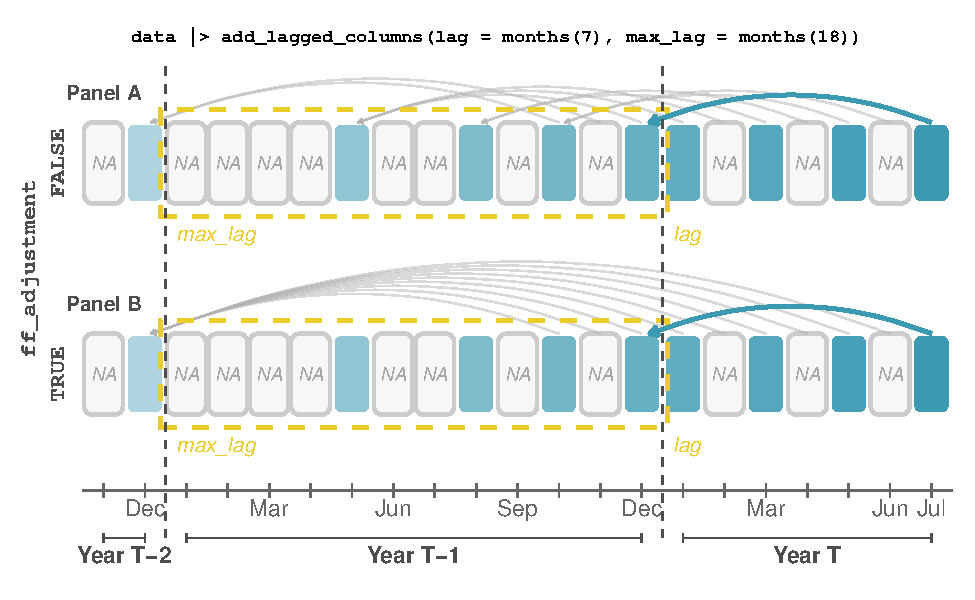
\includegraphics{jss-manuscript_files/figure-pdf/fig-lagging-illustration-1.pdf}

}

\caption{\label{fig-lagging-illustration}Two lagging mechanisms in
\texttt{add\_lagged\_columns()}. Each row represents a data series with
observed (filled) and missing (hollow) cells. Dashed rectangles mark the
search window; arrows show which value gets matched to each target
month.}

\end{figure}%

A handful of additional helpers cover routine operations that recur
across empirical studies. \texttt{winsorize()} and \texttt{trim()}
handle outliers in cross-sectional variables: the former replaces values
beyond user-specified quantiles with the quantile values themselves,
while the latter sets them to \texttt{NA}. \texttt{estimate\_model()}
fits a linear model from a formula string and returns the coefficients
as a tidy one-row data frame, which composes naturally with
\texttt{group\_by()} for grouped or rolling regressions such as
time-series factor exposures. \texttt{compute\_rolling\_value()} applies
an arbitrary aggregation function over a rolling window defined in
calendar time rather than row counts, accommodating irregular
observation frequencies and missing periods.

\subsubsection{Portfolio sorting}\label{sec-portfolio-sorting}

Portfolio sorts are among the most widely used tools in empirical asset
pricing (Bali, Engle, and Murray 2016). The procedure groups stocks each
period into portfolios based on a sorting variable, such as size, beta,
book-to-market, or momentum, and then compares return distributions
across the resulting portfolios. The long-short return between the
extreme portfolios is interpreted as a factor-mimicking strategy and
serves as the basis for tests of whether the sorting variable forecasts
future returns. We expose the procedure through four composable
functions.

\texttt{compute\_breakpoints()} takes a cross-section and a sorting
variable and returns the numeric cutoffs that define the portfolio
boundaries. The user supplies either a number of portfolios (for
example, five for quintiles) or an explicit vector of percentiles, but
not both. A \texttt{breakpoints\_exchanges} argument restricts the
universe used to compute breakpoints. The standard convention is
NYSE-only, which prevents the large cross-section of small NASDAQ firms
from dominating the lower bins. A related
\texttt{breakpoints\_min\_size\_threshold} argument excludes stocks
below a market-cap quantile from the breakpoint computation, which is
useful for size-related sorts where microcaps would otherwise distort
the cutoffs. A \texttt{smooth\_bunching} flag handles cases where the
sorting variable clusters at the edges by pinning extreme values to the
boundary portfolios and recomputing breakpoints on the remainder.

\texttt{assign\_portfolio()} maps each observation to a portfolio
integer using the breakpoints. The breakpoint computation is delegated
to a user-supplied function (defaulting to
\texttt{compute\_breakpoints()}), so custom rules such as dollar-based
cutoffs or industry-adjusted breakpoints can be plugged in without
rewriting the assignment logic. In practice,
\texttt{assign\_portfolio()} is called separately for each rebalancing
date, so that portfolios are reformed each period rather than fixed once
for the whole sample.

\texttt{compute\_portfolio\_returns()} ties the lower-level pieces
together into a single call. Given a panel of stock data, one or two
sorting variables, a sorting method, and \texttt{breakpoint\_options},
it handles rebalancing, breakpoint computation, portfolio assignment,
and return aggregation. It then returns a complete panel of portfolio
returns. For each portfolio-date the function reports three return
measures: equal-weighted, value-weighted using \texttt{mktcap\_lag} as
the weight, and capped value-weighted. The capped version pulls weights
above the \texttt{cap\_weight} percentile (default 0.8) back to that
cap, which prevents a small number of megacap firms from dominating the
portfolio. A \texttt{min\_portfolio\_size} argument sets the minimum
number of constituents below which the corresponding return is set to
\texttt{NA}. An optional \texttt{rebalancing\_month} argument switches
from period-by-period rebalancing to annual rebalancing in the specified
month. Portfolios formed in that month are then held constant for the
following twelve months.

The function supports three sorting schemes, illustrated in
Figure~\ref{fig-illustrate-portfolio-helper}. A \emph{univariate} sort
uses a single variable. An \emph{independent bivariate} sort computes
breakpoints on each variable separately and intersects the resulting
bins to produce a two-way grid. A \emph{dependent bivariate} sort first
partitions the cross-section by the secondary (control) variable and
then re-sorts within each bucket on the main variable, which is the
appropriate choice when the second variable is treated as a control
rather than as an independent dimension of variation. For bivariate
sorts, returns are averaged over the secondary variable so that only the
main-variable portfolios are returned.

\begin{figure}

\centering{

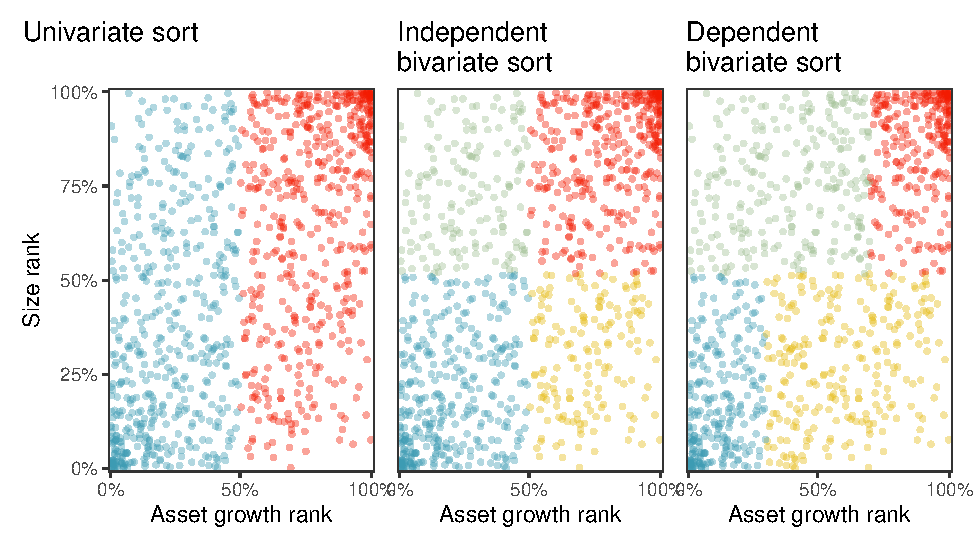
\includegraphics{jss-manuscript_files/figure-pdf/fig-illustrate-portfolio-helper-1.pdf}

}

\caption{\label{fig-illustrate-portfolio-helper}Portfolio sort
approaches illustrated for a single month (December 2024). Each panel
plots stock-month observations assigned to
\texttt{r\ .QuartoInlineRender(n\_portfolio)}×\texttt{r\ .QuartoInlineRender(n\_portfolio)}
portfolios based on asset growth rank (x-axis) and size rank (y-axis),
both expressed as percentiles. Colors indicate portfolio cell
assignment. The univariate sort (left) assigns portfolios on asset
growth alone; the independent bivariate sort (center) assigns each
dimension independently; the dependent bivariate sort (right) sorts on
size first, then on asset growth within size groups.}

\end{figure}%

\texttt{compute\_long\_short\_returns()} is a thin convenience layer
that takes the output of \texttt{compute\_portfolio\_returns()} and
computes the spread between the top and bottom portfolios. A
\texttt{direction} argument controls the sign and defaults to
\texttt{"top\_minus\_bottom"}. The function returns one long-short
series per return measure available in the input, so the equal-weighted,
value-weighted, and capped value-weighted spreads are produced in a
single call. This is the long-short factor-mimicking return that is
usually the object of interest in the asset-pricing literature.

\subsection{Vignette: A case study in factor construction}\label{sec-ag}

\begin{tcolorbox}[enhanced jigsaw, breakable, bottomrule=.15mm, titlerule=0mm, coltitle=black, left=2mm, opacitybacktitle=0.6, leftrule=.75mm, colframe=quarto-callout-note-color-frame, colback=white, toptitle=1mm, colbacktitle=quarto-callout-note-color!10!white, bottomtitle=1mm, arc=.35mm, title=\textcolor{quarto-callout-note-color}{\faInfo}\hspace{0.5em}{Note}, rightrule=.15mm, toprule=.15mm, opacityback=0]

This section shows the workflow from scratch without excessive
documentation by going through data aggregation, variable construction
for asset growth, lagging and sorting into portfolios. The purpose is to
illustrate the workflow and the relevant functions in a concrete
example. We do not show every step of the data cleaning process for
brevity.

\begin{itemize}
\tightlist
\item
  Compute asset growth risk factor time series once with defaults
  (describe the defaults) using \texttt{implement\_portfolio\_sort()}.
\item
  use the \texttt{filter\_options}, \texttt{breakpoint\_options}, and
  other arguments to streamline the process for an \emph{exotic}
  example.
\item
  Illustrate ``standard'' summary stats for one specification of the
  factor or use fama-mac beth functionality for some standard testing.
\end{itemize}

\end{tcolorbox}

We walk through the construction of the asset growth factor from raw
CRSP and Compustat data to long-short portfolio returns, implementing
each stage of Figure~\ref{fig-workflow-diagram} in turn. Each step uses
a \texttt{tidyfinance} function and generalises directly to any sorting
variable in the factor library.\footnote{Installation of the
  \texttt{tidyfinance} package is described in the appendix in
  Section~\ref{sec-installation} Installation and setup.}

Once installed, load \texttt{tidyfinance} and a minimal set of packages
for data manipulation and visualisation.

\begin{Shaded}
\begin{Highlighting}[]
\FunctionTok{library}\NormalTok{(}\StringTok{"tidyfinance"}\NormalTok{)}
\end{Highlighting}
\end{Shaded}

\begin{Shaded}
\begin{Highlighting}[]
\FunctionTok{library}\NormalTok{(}\StringTok{"dplyr"}\NormalTok{)}
\FunctionTok{library}\NormalTok{(}\StringTok{"tidyr"}\NormalTok{)}
\FunctionTok{library}\NormalTok{(}\StringTok{"lubridate"}\NormalTok{)}
\end{Highlighting}
\end{Shaded}

\subsubsection{Data download}\label{sec-data-download}

Before the first WRDS download, call \texttt{set\_wrds\_credentials()}
to store WRDS credentials securely in \texttt{.Renviron}; subsequent
\texttt{download\_data()} calls establish the database connection
automatically.

\begin{Shaded}
\begin{Highlighting}[]
\NormalTok{date\_start }\OtherTok{\textless{}{-}} \FunctionTok{as.Date}\NormalTok{(}\StringTok{"1960{-}01{-}01"}\NormalTok{)}
\NormalTok{date\_end }\OtherTok{\textless{}{-}} \FunctionTok{as.Date}\NormalTok{(}\StringTok{"2024{-}12{-}31"}\NormalTok{)}
\end{Highlighting}
\end{Shaded}

First, we download monthly stock returns from CRSP. Setting
\texttt{add\_ccm\_links\ =\ TRUE} appends CRSP-Compustat linking
identifiers needed to merge with financial statement data in the next
step.

\begin{Shaded}
\begin{Highlighting}[]
\NormalTok{crsp\_monthly }\OtherTok{\textless{}{-}} \FunctionTok{download\_data}\NormalTok{(}
  \AttributeTok{domain =} \StringTok{"wrds"}\NormalTok{,}
  \AttributeTok{dataset =} \StringTok{"crsp\_monthly"}\NormalTok{,}
  \AttributeTok{version =} \StringTok{"v2"}\NormalTok{,}
  \AttributeTok{start\_date =}\NormalTok{ date\_start,}
  \AttributeTok{end\_date =}\NormalTok{ date\_end,}
  \AttributeTok{add\_ccm\_links =} \ConstantTok{TRUE}
\NormalTok{)}
\end{Highlighting}
\end{Shaded}

The dataset contains 3451594 stock-month observations for 26263 unique
stocks, covering the period from 1960-01-01 to 2024-12-01.

Next, we download annual financial statements from Compustat.

\begin{Shaded}
\begin{Highlighting}[]
\NormalTok{compustat\_annual }\OtherTok{\textless{}{-}} \FunctionTok{download\_data}\NormalTok{(}
  \AttributeTok{domain =} \StringTok{"wrds"}\NormalTok{,}
  \AttributeTok{dataset =} \StringTok{"compustat\_annual"}\NormalTok{,}
  \AttributeTok{start\_date =}\NormalTok{ date\_start,}
  \AttributeTok{end\_date =}\NormalTok{ date\_end,}
  \AttributeTok{additional\_columns =} \FunctionTok{c}\NormalTok{(}\StringTok{"at"}\NormalTok{, }\StringTok{"ib"}\NormalTok{),}
  \AttributeTok{only\_us =} \ConstantTok{TRUE}
\NormalTok{)}
\end{Highlighting}
\end{Shaded}

Annual Compustat data contains 506778 firm-year observations for 39587
unique firms, covering the period from 1960-01-01 to 2024-12-01. The
\texttt{additional\_columns} argument retrieves total assets
(\texttt{at}) and income before extraordinary items (\texttt{ib}),
needed for computing asset growth and applying an earnings filter in
later steps. Setting \texttt{only\_us\ =\ TRUE} restricts the dataset to
USD-denominated observations, ensuring consistency with CRSP.

\subsubsection{Data cleaning and variable
construction}\label{sec-data-cleaning}

We illustrate data cleaning and variable construction using asset growth
(AG) as our running example. Asset growth is the year-over-year
percentage change in total assets (Cooper, Gulen, and Schill 2008), \[
AG_t = (AT_t - AT_{t-1}) / AT_{t-1}.
\]

The \texttt{add\_lagged\_columns()} function from \texttt{tidyfinance}
handles temporal alignment by creating a lagged version of total assets
grouped by firm identifier (\texttt{gvkey}) with a one-year lag.
Non-finite values (arising when lagged total assets are zero or missing)
become \texttt{NA}.\footnote{For the sake of simplicity we do not show
  every step of the data cleaning process in the paper. For instance, we
  apply an earnings filter to exclude firms with negative or zero income
  before extraordinary items (\texttt{ib}), which is a common practice
  in the literature to mitigate the influence of financial distress on
  asset growth portfolios. This filter is implemented in the code but
  not shown in the paper for brevity. We also apply an age filter to
  exclude firms younger than two years, which is common in the
  literature to ensure that the sorting variable is based on stable
  financial information. This filter is also implemented in the code but
  not shown in the paper for brevity. The factor library API provides
  preprocessed panels with all these filters applied, so users can
  access the final sorting variables without having to implement these
  steps themselves.}

\begin{Shaded}
\begin{Highlighting}[]
\NormalTok{sorting\_variable\_data }\OtherTok{\textless{}{-}}\NormalTok{ compustat\_annual }\SpecialCharTok{|\textgreater{}}
  \FunctionTok{add\_lagged\_columns}\NormalTok{(}
    \StringTok{"at"}\NormalTok{,}
    \AttributeTok{lag =} \FunctionTok{years}\NormalTok{(}\DecValTok{1}\NormalTok{),}
    \AttributeTok{by =} \StringTok{"gvkey"}\NormalTok{,}
\NormalTok{  ) }\SpecialCharTok{|\textgreater{}}
  \FunctionTok{mutate}\NormalTok{(}
    \AttributeTok{asset\_growth =}\NormalTok{ (at }\SpecialCharTok{{-}}\NormalTok{ at\_lag) }\SpecialCharTok{/}\NormalTok{ at\_lag,}
    \AttributeTok{asset\_growth =} \FunctionTok{if\_else}\NormalTok{(}\FunctionTok{is.finite}\NormalTok{(asset\_growth), asset\_growth, }\ConstantTok{NA\_real\_}\NormalTok{)}
\NormalTok{  ) }\SpecialCharTok{|\textgreater{}}
  \FunctionTok{select}\NormalTok{(gvkey, date, asset\_growth)}
\end{Highlighting}
\end{Shaded}

\texttt{sorting\_variable\_data} contains one observation per firm-year,
the natural unit for cross-sectional analysis of annual accounting
variables. The package provides \texttt{filter\_out()} as a convenience
wrapper that removes rows matching a logical predicate, and
\texttt{winsorize()} to clip numeric vectors at specified quantile
bounds. Asset growth is heavily right-skewed: a small number of firms
with dramatic balance-sheet expansions generate extreme positive values.
We winsorize at the 1st and 99th percentiles before computing summary
statistics. Table~\ref{tbl-ag-summary} reports the pooled
cross-sectional summary; Table~\ref{tbl-ag-summary-yearly} shows how
those moments vary across calendar years.

\begin{longtable}[]{@{}rrrrrrrr@{}}

\caption{\label{tbl-ag-summary}Cross-sectional summary statistics for
asset growth (winsorized at the 1st and 99th percentiles). The table
reports the number of firm-year observations (N), the mean, standard
deviation (SD), and selected percentiles of the annual asset growth
distribution computed from \texttt{sorting\_variable\_data}.}

\tabularnewline

\toprule\noalign{}
N & Mean & SD & P10 & P25 & Median & P75 & P90 \\
\midrule\noalign{}
\endhead
\bottomrule\noalign{}
\endlastfoot
389123 & 0.238 & 0.858 & -0.191 & -0.034 & 0.064 & 0.207 & 0.588 \\

\end{longtable}

\begin{longtable}[]{@{}
  >{\raggedleft\arraybackslash}p{(\columnwidth - 16\tabcolsep) * \real{0.0645}}
  >{\raggedleft\arraybackslash}p{(\columnwidth - 16\tabcolsep) * \real{0.0645}}
  >{\raggedleft\arraybackslash}p{(\columnwidth - 16\tabcolsep) * \real{0.1183}}
  >{\raggedleft\arraybackslash}p{(\columnwidth - 16\tabcolsep) * \real{0.1183}}
  >{\raggedleft\arraybackslash}p{(\columnwidth - 16\tabcolsep) * \real{0.1183}}
  >{\raggedleft\arraybackslash}p{(\columnwidth - 16\tabcolsep) * \real{0.0968}}
  >{\raggedleft\arraybackslash}p{(\columnwidth - 16\tabcolsep) * \real{0.1398}}
  >{\raggedleft\arraybackslash}p{(\columnwidth - 16\tabcolsep) * \real{0.1398}}
  >{\raggedleft\arraybackslash}p{(\columnwidth - 16\tabcolsep) * \real{0.1398}}@{}}

\caption{\label{tbl-ag-summary-yearly}Time-series averages of annual
cross-sectional summary statistics for asset growth (winsorized at the
1st and 99th percentiles). For each calendar year, cross-sectional mean,
standard deviation, and median are computed from
\texttt{sorting\_variable\_data}; the table reports the time-series
mean, minimum, and maximum of those annual statistics.}

\tabularnewline

\toprule\noalign{}
\begin{minipage}[b]{\linewidth}\raggedleft
Years
\end{minipage} & \begin{minipage}[b]{\linewidth}\raggedleft
Avg N
\end{minipage} & \begin{minipage}[b]{\linewidth}\raggedleft
Mean (avg)
\end{minipage} & \begin{minipage}[b]{\linewidth}\raggedleft
Mean (min)
\end{minipage} & \begin{minipage}[b]{\linewidth}\raggedleft
Mean (max)
\end{minipage} & \begin{minipage}[b]{\linewidth}\raggedleft
SD (avg)
\end{minipage} & \begin{minipage}[b]{\linewidth}\raggedleft
Median (avg)
\end{minipage} & \begin{minipage}[b]{\linewidth}\raggedleft
Median (min)
\end{minipage} & \begin{minipage}[b]{\linewidth}\raggedleft
Median (max)
\end{minipage} \\
\midrule\noalign{}
\endhead
\bottomrule\noalign{}
\endlastfoot
64 & 6080 & 0.242 & 0.048 & 0.889 & 0.847 & 0.067 & 0.001 & 0.132 \\

\end{longtable}

The next step merges annual sorting variables onto the monthly CRSP
stock panel using \texttt{join\_lagged\_values()}. The function aligns
fiscal-year-end data with monthly observations through a configurable
lag window. Setting \texttt{ff\_adjustment\ =\ TRUE} implements the
Fama-French convention (Eugene F. Fama and French 1993), aligning
fiscal-year data from year \(t\) with portfolio formation in July of
year \(t+1\) through a 12-to-18-month look-back window. The same lagging
process generalizes to all sorting variables in the full factor library.
The factor library API provides precomputed lagged panels for all
variables.

With both lagging mechanisms documented, we apply
\texttt{join\_lagged\_values()} to merge the sorting variable onto the
monthly return panel. Figure~\ref{fig-ag-percentiles} shows the 33rd,
50th, and 66th percentiles of asset growth over time in the resulting
panel; pronounced spikes during economic expansions and contractions
highlight the cyclical nature of corporate investment that portfolio
sorts aim to exploit.

\begin{Shaded}
\begin{Highlighting}[]
\NormalTok{sorting\_data }\OtherTok{\textless{}{-}}\NormalTok{ crsp\_monthly }\SpecialCharTok{|\textgreater{}}
  \FunctionTok{join\_lagged\_values}\NormalTok{(}
\NormalTok{    sorting\_variable\_data,}
    \StringTok{"gvkey"}\NormalTok{,}
    \AttributeTok{min\_lag =} \FunctionTok{months}\NormalTok{(}\DecValTok{7}\NormalTok{),}
    \AttributeTok{max\_lag =} \FunctionTok{months}\NormalTok{(}\DecValTok{18}\NormalTok{),}
    \AttributeTok{ff\_adjustment =} \ConstantTok{TRUE}
\NormalTok{  )}

\NormalTok{sorting\_data }\OtherTok{\textless{}{-}}\NormalTok{ sorting\_data }\SpecialCharTok{|\textgreater{}}
  \FunctionTok{select}\NormalTok{(date, permno, exchange, ret\_excess, mktcap\_lag, asset\_growth) }\SpecialCharTok{|\textgreater{}}
  \FunctionTok{filter}\NormalTok{(date }\SpecialCharTok{\textgreater{}}\NormalTok{ date\_start }\SpecialCharTok{+} \FunctionTok{months}\NormalTok{(}\DecValTok{12}\NormalTok{) }\SpecialCharTok{+} \FunctionTok{months}\NormalTok{(}\DecValTok{18}\NormalTok{))}
\end{Highlighting}
\end{Shaded}

The filter removes the initial year used to compute the growth rate and
an additional 18 months to avoid mechanically introduced gaps from the
lagging step, leaving a panel of stock-month observations with excess
returns, exchange membership, lagged market capitalization, and the
lagged sorting variable.

\begin{figure}

\centering{

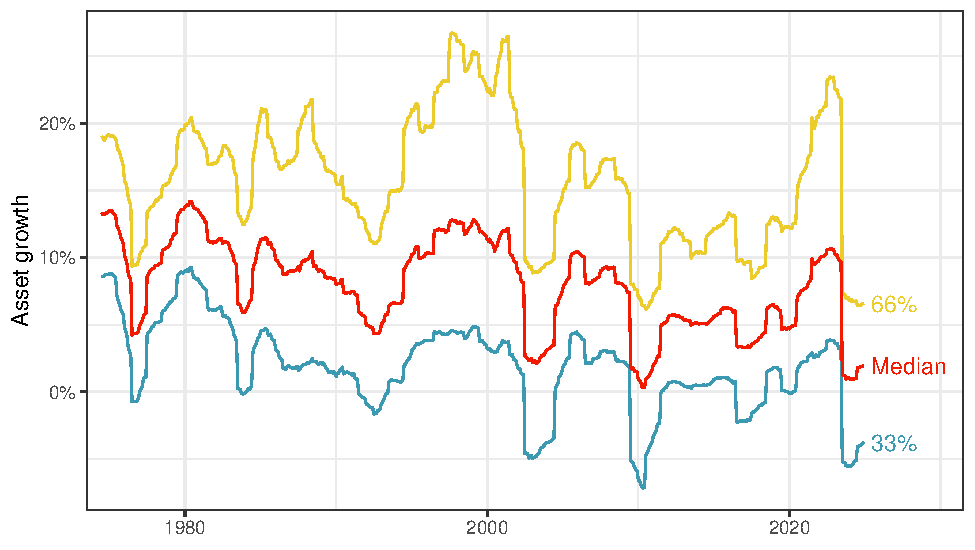
\includegraphics{jss-manuscript_files/figure-pdf/fig-ag-percentiles-1.pdf}

}

\caption{\label{fig-ag-percentiles}Distribution of asset growth over
time. Lines show the 33rd, 50th, and 66th percentiles of the
cross-sectional distribution of asset growth in \texttt{sorting\_data},
the firm-month panel used as input for portfolio construction. Asset
growth is expressed as a proportion (e.g., 0.2 = 20\% annual growth in
total assets) and covers the full sample period of the merged
CRSP-Compustat dataset.}

\end{figure}%

With the sorting variable constructed and merged onto the monthly stock
panel, we now turn to portfolio sorts, the mechanism that translates
firm-level characteristics into tradable factor returns.

\subsubsection{Portfolio sorts}\label{sec-portfolio-sorts}

In portfolio sorts, stocks are ranked each period by their sorting
variable and divided into quantile portfolios. Portfolio returns are
equal-weighted or value-weighted averages of constituent stock returns.
The long-short factor return is the difference between the extreme
portfolios, for instance bottom minus top for asset growth, reflecting
the negative premium documented by Cooper, Gulen, and Schill (2008). Key
methodological decisions include the number of portfolios, the exchange
universe for computing breakpoints, the weighting scheme, and the
rebalancing frequency.

The \texttt{tidyfinance} package implements this workflow through three
functions. First, \texttt{breakpoint\_options()} configures the sorting
parameters: the number of quantile portfolios and which exchanges
determine the breakpoints. Second,
\texttt{compute\_portfolio\_returns()} takes the sorting data, applies
the specified configuration, and returns portfolio-level returns. Third,
\texttt{compute\_long\_short\_returns()} constructs the hedge portfolio
return from the extreme quantiles.

\paragraph{Univariate sorts}\label{sec-univariate-sorts}

\texttt{compute\_portfolio\_returns()} is built on two lower-level
functions that are also available for custom workflows.
\texttt{compute\_breakpoints()} computes quantile cutpoints for the
sorting variable from a specified exchange universe.
\texttt{assign\_portfolio()} maps each stock-month to a portfolio number
based on those cutpoints. Researchers who need finer control, for
instance to build overlapping portfolios, apply non-standard cutoffs, or
weight within cells differently, can call these functions directly
rather than through the high-level wrapper.

In a univariate sort, stocks are ranked on a single characteristic. We
illustrate this with asset growth, forming decile portfolios using NYSE
breakpoints and value-weighted returns, rebalanced annually in July.

\begin{Shaded}
\begin{Highlighting}[]
\NormalTok{options\_main }\OtherTok{\textless{}{-}} \FunctionTok{breakpoint\_options}\NormalTok{(}
  \AttributeTok{n\_portfolios =} \DecValTok{5}\NormalTok{,}
  \AttributeTok{breakpoint\_exchanges =} \StringTok{"NYSE"}
\NormalTok{)}
\end{Highlighting}
\end{Shaded}

The \texttt{breakpoint\_options()} call specifies that breakpoints come
from NYSE-listed stocks only, a common convention that avoids the
influence of small AMEX and NASDAQ firms on portfolio cutoffs. We then
pass these options to \texttt{compute\_portfolio\_returns()}.

\begin{Shaded}
\begin{Highlighting}[]
\NormalTok{portfolio\_returns }\OtherTok{\textless{}{-}} \FunctionTok{compute\_portfolio\_returns}\NormalTok{(}
\NormalTok{  sorting\_data,}
  \AttributeTok{sorting\_variables =} \StringTok{"asset\_growth"}\NormalTok{,}
  \AttributeTok{sorting\_method =} \StringTok{"univariate"}\NormalTok{,}
  \AttributeTok{rebalancing\_month =} \DecValTok{7}\NormalTok{,}
\NormalTok{  options\_main}
\NormalTok{)}
\end{Highlighting}
\end{Shaded}

\begin{verbatim}
Returning a complete panel with 55 missing values in factor returns due to
insufficient observations (n() < 0).
\end{verbatim}

\texttt{compute\_portfolio\_returns()} returns a long tibble with one
row per portfolio-month, containing value-weighted
(\texttt{ret\_excess\_vw}), equal-weighted (\texttt{ret\_excess\_ew}),
and capped value-weighted (\texttt{ret\_excess\_vw\_capped}) excess
returns. The long-short factor return is obtained via
\texttt{compute\_long\_short\_returns()}. The
\texttt{direction\ =\ "bottom\_minus\_top"} argument means the factor is
long low-AG stocks and short high-AG stocks, consistent with the
negative premium documented by Cooper, Gulen, and Schill (2008).

\begin{Shaded}
\begin{Highlighting}[]
\NormalTok{factor\_returns\_ag }\OtherTok{\textless{}{-}}\NormalTok{ portfolio\_returns }\SpecialCharTok{|\textgreater{}}
  \FunctionTok{compute\_long\_short\_returns}\NormalTok{(}\AttributeTok{direction =} \StringTok{"bottom\_minus\_top"}\NormalTok{)}
\end{Highlighting}
\end{Shaded}

Table~\ref{tbl-univariate-sort-ag} summarises the time series of each
quintile across all three weighting schemes, with the long-short
portfolio appended as the final row.

\begin{longtable}[]{@{}
  >{\raggedright\arraybackslash}p{(\columnwidth - 12\tabcolsep) * \real{0.1515}}
  >{\raggedleft\arraybackslash}p{(\columnwidth - 12\tabcolsep) * \real{0.1212}}
  >{\raggedleft\arraybackslash}p{(\columnwidth - 12\tabcolsep) * \real{0.1515}}
  >{\raggedleft\arraybackslash}p{(\columnwidth - 12\tabcolsep) * \real{0.1212}}
  >{\raggedleft\arraybackslash}p{(\columnwidth - 12\tabcolsep) * \real{0.1515}}
  >{\raggedleft\arraybackslash}p{(\columnwidth - 12\tabcolsep) * \real{0.1364}}
  >{\raggedleft\arraybackslash}p{(\columnwidth - 12\tabcolsep) * \real{0.1667}}@{}}

\caption{\label{tbl-univariate-sort-ag}Time-series averages of
annualised monthly excess returns for asset growth quintile portfolios.
Portfolios are formed annually in July using NYSE breakpoints,
rebalanced annually. Means are annualised (multiplied by 12). The
\(t\)\textasciitilde statistic tests whether the mean monthly excess
return differs from zero. The L/S row is the long-short portfolio
(bottom minus top quintile).}

\tabularnewline

\toprule\noalign{}
\begin{minipage}[b]{\linewidth}\raggedright
Portfolio
\end{minipage} & \begin{minipage}[b]{\linewidth}\raggedleft
VW Mean
\end{minipage} & \begin{minipage}[b]{\linewidth}\raggedleft
VW t-stat
\end{minipage} & \begin{minipage}[b]{\linewidth}\raggedleft
EW Mean
\end{minipage} & \begin{minipage}[b]{\linewidth}\raggedleft
EW t-stat
\end{minipage} & \begin{minipage}[b]{\linewidth}\raggedleft
VWC Mean
\end{minipage} & \begin{minipage}[b]{\linewidth}\raggedleft
VWC t-stat
\end{minipage} \\
\midrule\noalign{}
\endhead
\bottomrule\noalign{}
\endlastfoot
1 & 0.093 & 4.349 & 0.149 & 4.816 & 0.103 & 4.085 \\
2 & 0.079 & 4.343 & 0.117 & 5.139 & 0.095 & 4.530 \\
3 & 0.071 & 3.796 & 0.108 & 4.845 & 0.092 & 4.425 \\
4 & 0.073 & 3.677 & 0.103 & 4.297 & 0.088 & 3.935 \\
5 & 0.067 & 2.667 & 0.050 & 1.630 & 0.056 & 1.981 \\
L/S & 0.026 & 1.924 & 0.099 & 9.116 & 0.047 & 4.468 \\

\end{longtable}

The value-weighted long-short portfolio earns 2.6\% per year
(\(t\)\textasciitilde statistic 1.92), consistent with the negative
premium documented by Cooper, Gulen, and Schill (2008). The
equal-weighted spread is larger, as expected for characteristics that
correlate with size. The monotone decline across quintiles confirms that
\texttt{tidyfinance} reproduces the literature result from raw WRDS
data.

\paragraph{Bivariate sorts}\label{sec-bivariate-sorts}

Bivariate (double) sorts control for a second variable, typically firm
size (\texttt{mktcap\_lag}), when forming portfolios. In dependent
sorts, stocks are first sorted into groups by the secondary variable;
within each group, they are then sorted on the main characteristic. In
independent sorts, both sorts apply unconditionally, and portfolios form
at the intersections. The factor return averages across the secondary
dimension, isolating the effect of the primary variable after
controlling for size. Figure~\ref{fig-illustrate-portfolio-helper}
illustrates the three approaches for a single cross-section.

We reuse \texttt{options\_main} from the univariate sort (five
portfolios, NYSE breakpoints) and add a separate options object for the
secondary size dimension:

\begin{Shaded}
\begin{Highlighting}[]
\NormalTok{options\_secondary }\OtherTok{\textless{}{-}} \FunctionTok{breakpoint\_options}\NormalTok{(}
  \AttributeTok{n\_portfolios =} \DecValTok{2}\NormalTok{,}
  \AttributeTok{breakpoint\_exchanges =} \StringTok{"NYSE"}
\NormalTok{)}

\NormalTok{portfolio\_returns\_biv }\OtherTok{\textless{}{-}} \FunctionTok{compute\_portfolio\_returns}\NormalTok{(}
\NormalTok{  sorting\_data,}
  \FunctionTok{c}\NormalTok{(}\StringTok{"asset\_growth"}\NormalTok{, }\StringTok{"mktcap\_lag"}\NormalTok{),}
  \AttributeTok{sorting\_method =} \StringTok{"bivariate{-}dependent"}\NormalTok{,}
  \AttributeTok{rebalancing\_month =} \DecValTok{7}\NormalTok{,}
\NormalTok{  options\_main,}
\NormalTok{  options\_secondary}
\NormalTok{)}
\end{Highlighting}
\end{Shaded}

\begin{verbatim}
Returning a complete panel with 55 missing values in factor returns due to
insufficient observations (n() < 0).
\end{verbatim}

\begin{Shaded}
\begin{Highlighting}[]
\NormalTok{factor\_returns\_biv }\OtherTok{\textless{}{-}}\NormalTok{ portfolio\_returns\_biv }\SpecialCharTok{|\textgreater{}}
  \FunctionTok{compute\_long\_short\_returns}\NormalTok{(}\AttributeTok{direction =} \StringTok{"bottom\_minus\_top"}\NormalTok{)}
\end{Highlighting}
\end{Shaded}

\begin{longtable}[]{@{}lrr@{}}

\caption{\label{tbl-bivariate-comparison}Univariate vs size-controlled
long-short returns for asset growth. Annualized value-weighted mean
excess return and \(t\)\textasciitilde statistic for the univariate sort
and the dependent bivariate sort averaging across two size groups.
Portfolios use NYSE breakpoints and annual July rebalancing.}

\tabularnewline

\toprule\noalign{}
Sort & VW Mean & VW \(t\)\textasciitilde stat \\
\midrule\noalign{}
\endhead
\bottomrule\noalign{}
\endlastfoot
Univariate & 0.026 & 1.924 \\
Bivariate (size-controlled) & 0.036 & 3.376 \\

\end{longtable}

The AG premium survives size control, suggesting it captures an
investment effect distinct from the size factor. The
\texttt{sorting\_method} argument switches between dependent and
independent double sorts, so researchers can inspect both configurations
without modifying the pipeline.

\subsection{Factor library and API}\label{sec-library}

\begin{tcolorbox}[enhanced jigsaw, breakable, bottomrule=.15mm, titlerule=0mm, coltitle=black, left=2mm, opacitybacktitle=0.6, leftrule=.75mm, colframe=quarto-callout-note-color-frame, colback=white, toptitle=1mm, colbacktitle=quarto-callout-note-color!10!white, bottomtitle=1mm, arc=.35mm, title=\textcolor{quarto-callout-note-color}{\faInfo}\hspace{0.5em}{Note}, rightrule=.15mm, toprule=.15mm, opacityback=0]

This section introduces the full factor library and API.

\begin{itemize}
\tightlist
\item
  Explain the computation of the entire grid of factor returns across
  all combinations of methodological choices. Cite WWW and Gruber et
  al.~for the motivation of this comprehensive approach.
\item
  Emphasise that the library is available for download, so researchers
  can access results without re-running the computationally intensive
  portfolio sort pipeline.
\item
  Show how to download one default time series and how to use
  \texttt{fill\_all}.
\item
  Illustrate Sharpe-ratio variation.
\item
  Mention that ´py-tidyfinance` can be used with identical callss
\end{itemize}

\end{tcolorbox}

\subsubsection{Specification grid}\label{sec-specification-grid}

The examples above represent single points in a high-dimensional space
of methodological choices. Table~\ref{tbl-sorting-decisions} summarises
the preprocessing decisions that can be varied when constructing factor
returns. The full factor library exhaustively evaluates all valid
combinations of these choices for each of the sorting variables listed
in Table~\ref{tbl-sorting-variables}.

\begin{longtable}[]{@{}
  >{\raggedright\arraybackslash}p{(\columnwidth - 6\tabcolsep) * \real{0.1371}}
  >{\raggedright\arraybackslash}p{(\columnwidth - 6\tabcolsep) * \real{0.1878}}
  >{\raggedright\arraybackslash}p{(\columnwidth - 6\tabcolsep) * \real{0.2640}}
  >{\raggedright\arraybackslash}p{(\columnwidth - 6\tabcolsep) * \real{0.4112}}@{}}

\caption{\label{tbl-sorting-decisions}Preprocessing choices in the
portfolio sort grid and corresponding \texttt{download\_data()}
arguments. Italic values indicate the default. For double sorts, the
secondary quantiles and exchange choices apply to the size dimension
only; for univariate sorts, those rows are not applicable. FF refers to
the lag procedure of Eugene F. Fama and French (1993).}

\tabularnewline

\toprule\noalign{}
\begin{minipage}[b]{\linewidth}\raggedright
Preprocessing choice
\end{minipage} & \begin{minipage}[b]{\linewidth}\raggedright
Argument
\end{minipage} & \begin{minipage}[b]{\linewidth}\raggedright
Options
\end{minipage} & \begin{minipage}[b]{\linewidth}\raggedright
Description
\end{minipage} \\
\midrule\noalign{}
\endhead
\bottomrule\noalign{}
\endlastfoot
Size exclusion & \texttt{exclude\_size} & None; \emph{bottom 20\%} &
Fraction of the smallest stocks (by NYSE market cap) excluded from the
universe. \\
Exclusion of financials & \texttt{exclude\_financials} & \emph{No}; Yes
& Drops financial-sector stocks (SIC 6000--6999) from the universe. \\
Exclusion of utilities & \texttt{exclude\_utilities} & \emph{No}; Yes &
Drops utility-sector stocks (SIC 4900--4999) from the universe. \\
Exclusion of neg. earnings & \texttt{exclude\_negative\_earnings} &
\emph{No}; Yes & Drops firms with negative earnings before sorting. \\
Sorting variable lag & \texttt{sorting\_variable\_lag} & 3m; \emph{6m};
FF & Lag applied to the sorting variable before portfolio assignment. \\
Rebalancing & \texttt{rebalancing} & \emph{Monthly}; Annual & How
frequently portfolios are reformed. \\
BP: Quantiles (main) & \texttt{breakpoints\_main} & 3; 5; \emph{10} &
Number of quantile groups for the portfolio sort. \\
Sort method & \texttt{sorting\_method} & \emph{Single}; Double
dependent; Double independent & Single sort or sequential double sort
(by size). \\
BP: Quantiles (secondary) & \texttt{breakpoints\_secondary} & \emph{NA};
2; 5 & Groups for the secondary sort variable; only relevant for double
sorts. \\
BP: Exchanges & \texttt{breakpoints\_exchanges} & \emph{NYSE}; All &
Exchange(s) used to compute quantile breakpoints. \\
Weighting scheme & \texttt{weighting\_scheme} & EW; \emph{VW}; truncated
VW & Return weighting within portfolios. \\

\end{longtable}

We host precomputed factor returns for all specifications on Hugging
Face and make them accessible via the \texttt{tidyfinance} API.
Researchers can retrieve results without re-running the computationally
intensive portfolio sort pipeline. An interactive download interface is
also available at
\href{https://factors.tidy-finance.org}{factors.tidy-finance.org}.

The factor library covers 50 sorting variables across seven categories:
investment, profitability, valuation, momentum, intangibles, trading
frictions, and financing. The selection follows Jensen, Kelly, and
Pedersen (2023). Table~\ref{tbl-sorting-variables} lists all variables
with their long-short direction and primary reference.

\subsubsection{The factor library}\label{sec-library-practice}

This sensitivity is not specific to AG. For all 50 sorting variables in
the library, construction choices shift Sharpe ratios by enough to
reverse the sign of the premium for some factors.
Figure~\ref{fig-sharpe-ratio} shows the distribution of annualized
Sharpe ratios for each variable across all 187008 specifications.

\begin{figure}[p]

\centering{

\includegraphics[width=1\textwidth,height=\textheight]{jss-manuscript_files/figure-pdf/fig-sharpe-ratio-1.pdf}

}

\caption{\label{fig-sharpe-ratio}Sharpe ratios across construction
choices. Ridge plots show the distribution of annualized Sharpe ratios
of long-short return differentials for each sorting variable across all
\texttt{r\ .QuartoInlineRender(nrow(portfolio\_sort\_grid))}
specifications illustrated in Table~\ref{tbl-sorting-decisions}, based
on the available sample period per factor. Most variables exhibit
substantial variation across specifications, underscoring the
sensitivity of factor returns to construction choices.}

\end{figure}%

Figure~\ref{fig-sharpe-ratio} conveys two findings. First, most
distributions are wide: construction choices have material effects on
factor performance across the library. Second, for several factors the
distribution spans zero, meaning the premium's sign depends on the
specification. A researcher reporting a single undocumented series risks
mistaking a construction artifact for an economic signal. Factors with
narrow distributions centered well above zero are construction-robust;
those with wide or zero-straddling distributions require sensitivity
analysis before drawing conclusions.

Table~\ref{tbl-sorting-variables} lists all 50 sorting variables with
their long-short direction and primary reference.

\begin{longtable}{lp{5cm}ll}

\caption{\label{tbl-sorting-variables}Sorting variables in the factor
library. The direction column indicates whether the long-short factor
return goes long top-minus-bottom (↑) or bottom-minus-top (↓) of the
characteristic distribution.}

\tabularnewline

\toprule
Variable & Name &  & Main reference\\
\midrule
sv_52w & 52-Week High & $\uparrow$ & \cite{george.2004}\\
sv_aci & Abnormal Corporate Investment & $\downarrow$ & \cite{titman.2004}\\
sv_ami & Amihud Illiquidity & $\uparrow$ & \cite{amihud.2002}\\
sv_ag & Asset Growth & $\downarrow$ & \cite{cooper.2008}\\
sv_beta & Beta & $\uparrow$ & \cite{fama.1973}\\
\addlinespace
sv_bm & Book-to-Market & $\uparrow$ & \cite{daniel.2006}\\
sv_cfm & Cash Flow to Market & $\uparrow$ & \cite{lakonishok.1994}\\
sv_cbop & Cash-Based Operating Profitability & $\uparrow$ & \cite{ball.2016}\\
sv_dbe & Change in Common Equity & $\downarrow$ & \cite{richardson.2005}\\
sv_dcol & Change in Current Operating Liabilities & $\downarrow$ & \cite{richardson.2005}\\
\addlinespace
sv_dfnl & Change in Financial Liabilities & $\downarrow$ & \cite{richardson.2005}\\
sv_dnoa & Change in Net Operating Assets & $\downarrow$ & \cite{hirshleifer.2004}\\
sv_dpia & Change in PPE and Intangibles & $\downarrow$ & \cite{lyandres.2008}\\
sv_dwc & Change in Working Capital & $\downarrow$ & \cite{richardson.2005}\\
sv_cdi & Composite Debt Issuance & $\downarrow$ & \cite{lyandres.2008}\\
\addlinespace
sv_csi & Composite Share Issuance & $\downarrow$ & \cite{daniel.2006}\\
sv_dm & Debt to Market & $\uparrow$ & \cite{bhandari.1988}\\
sv_dtv & Dollar Trading Volume & $\downarrow$ & \cite{brennan.1998}\\
sv_em & Earnings to Market & $\uparrow$ & \cite{basu.1983}\\
sv_ebm & Enterprise Book to Market & $\uparrow$ & \cite{penman.2007}\\
\addlinespace
sv_gpa & Gross Profit Asset & $\uparrow$ & \cite{novy-marx.2013}\\
sv_hr & Hiring Rate & $\downarrow$ & \cite{belo.2012}\\
sv_iskew & Idiosyncratic Skewness & $\downarrow$ & \cite{bali.2016}\\
sv_ivol & Idiosyncratic Volatility & $\downarrow$ & \cite{ang.2006}\\
sv_dinv & Inventory Changes & $\downarrow$ & \cite{thomas.2002}\\
\addlinespace
sv_ig & Investment Growth & $\downarrow$ & \cite{xing.2008}\\
sv_rev & Long-Term Reversal & $\downarrow$ & \cite{debondt.1985}\\
sv_me & Market Equity & $\downarrow$ & \cite{banz.1981}\\
sv_mdr & Maximum Daily Return & $\downarrow$ & \cite{bali.2011}\\
sv_mom & Momentum & $\uparrow$ & \cite{fama.1996}\\
\addlinespace
sv_ndf & Net Debt Financing & $\downarrow$ & \cite{baker.2006}\\
sv_ndm & Net Debt to Market & $\downarrow$ & \cite{penman.2007}\\
sv_nef & Net Equity Financing & $\downarrow$ & \cite{baker.2006}\\
sv_nxf & Net External Financing & $\downarrow$ & \cite{baker.2006}\\
sv_noa & Net Operating Assets & $\downarrow$ & \cite{hirshleifer.2004}\\
\addlinespace
sv_npy & Net Payout Yield & $\uparrow$ & \cite{boudoukh.2007}\\
sv_o & O-Score & $\downarrow$ & \cite{ohlson.1980,dichev.1998}\\
sv_oa & Operating Accruals & $\downarrow$ & \cite{sloan.1996}\\
sv_ocm & Operating Cash Flow to Market & $\uparrow$ & \cite{desai.2004}\\
sv_ope & Operating Efficiency & $\uparrow$ & \cite{fama.2015}\\
\addlinespace
sv_ol & Operating Leverage & $\uparrow$ & \cite{novy-marx.2011}\\
sv_rer & Real-Estate Ratio & $\uparrow$ & \cite{titman.2004}\\
sv_rs & Relative Strength & $\uparrow$ & \cite{jegadeesh.2006}\\
sv_rmom & Residual Momentum & $\uparrow$ & \cite{blitz.2011}\\
sv_roa & Return on Assets & $\uparrow$ & \cite{balakrishnan.2010}\\
\addlinespace
sv_roe & Return on Equity & $\uparrow$ & \cite{hou.2014}\\
sv_sm & Sales to Market & $\uparrow$ & \cite{barbee.1996}\\
sv_tur & Share Turnover & $\downarrow$ & \cite{datar.1998}\\
sv_sue & Standardized Unexpected Earnings & $\uparrow$ & \cite{foster.1984}\\
sv_tbi & Taxable Income to Book Income & $\downarrow$ & \cite{lev.2004}\\
\bottomrule

\end{longtable}

To download factor returns from the factor library, call

\begin{Shaded}
\begin{Highlighting}[]
\NormalTok{asset\_growth\_returns }\OtherTok{\textless{}{-}} \FunctionTok{download\_data}\NormalTok{(}
  \StringTok{"tidyfinance"}\NormalTok{,}
  \StringTok{"factor\_library"}\NormalTok{,}
  \AttributeTok{sorting\_variable =} \StringTok{"ag"}\NormalTok{,}
  \AttributeTok{sorting\_variable\_lag =} \StringTok{"6m"}
\NormalTok{)}
\end{Highlighting}
\end{Shaded}

The defaults passed to \texttt{dataset\ =\ "factor\_library"} reflect
one common construction choice but may not suit every research question.
Always verify that the selected combination matches the intended design
before drawing conclusions.

\begin{Shaded}
\begin{Highlighting}[]
\FunctionTok{download\_data}\NormalTok{(}
  \StringTok{"tidyfinance"}\NormalTok{,}
  \StringTok{"factor\_library"}\NormalTok{,}
  \AttributeTok{sorting\_variable =} \StringTok{"52w"}\NormalTok{,}
  \AttributeTok{sorting\_variable\_lag =} \StringTok{"6m"}\NormalTok{,}
  \AttributeTok{fill\_all =} \ConstantTok{TRUE}
\NormalTok{)}
\end{Highlighting}
\end{Shaded}

For finer control, \texttt{tidyfinance} exposes lower-level helpers that
sit beneath the \texttt{download\_data()} interface.
\texttt{get\_available\_huggingface\_files()} returns all available
files for a given Hugging Face repository as a tibble;
\texttt{download\_factor\_library\_returns\_ids()} retrieves returns for
a specific vector of precomputed specification IDs. Researchers who want
to iterate over a custom subset of specifications rather than filter by
parameter value will prefer this route.

\begin{Shaded}
\begin{Highlighting}[]
\NormalTok{full\_grid }\OtherTok{\textless{}{-}} \FunctionTok{get\_available\_huggingface\_files}\NormalTok{(}
  \StringTok{"tidy{-}finance"}\NormalTok{,}
  \StringTok{"factor{-}library{-}grid"}
\NormalTok{) }\SpecialCharTok{|\textgreater{}}
\NormalTok{  dplyr}\SpecialCharTok{::}\FunctionTok{pull}\NormalTok{(.data}\SpecialCharTok{$}\NormalTok{url) }\SpecialCharTok{|\textgreater{}}
\NormalTok{  arrow}\SpecialCharTok{::}\FunctionTok{read\_parquet}\NormalTok{()}

\FunctionTok{download\_factor\_library\_returns\_ids}\NormalTok{(}\FunctionTok{c}\NormalTok{(}\DecValTok{123}\NormalTok{, }\DecValTok{456}\NormalTok{))}
\end{Highlighting}
\end{Shaded}

\subsection{Summary and discussion}\label{sec-summary}

\begin{tcolorbox}[enhanced jigsaw, breakable, bottomrule=.15mm, titlerule=0mm, coltitle=black, left=2mm, opacitybacktitle=0.6, leftrule=.75mm, colframe=quarto-callout-note-color-frame, colback=white, toptitle=1mm, colbacktitle=quarto-callout-note-color!10!white, bottomtitle=1mm, arc=.35mm, title=\textcolor{quarto-callout-note-color}{\faInfo}\hspace{0.5em}{Note}, rightrule=.15mm, toprule=.15mm, opacityback=0]

Keep brief or delete entirely, as the main paper's conclusion already
covers the key points.

\end{tcolorbox}

Factor returns encode their construction history. Two researchers
following the same paper can produce different factor series, with no
way of knowing why, because breakpoints, weighting, and lagging
conventions are rarely published alongside the data.
\texttt{tidyfinance} makes these decisions visible: the package covers
50 sorting variables across 187008 documented specifications, each
reproducible from raw WRDS and Compustat data in a single,
version-controlled workflow.

The library currently covers US equities. Construction-choice
sensitivity in international markets is beyond its current scope.

The broader implication is methodological. Researchers who disagree
about a construction choice can resolve the disagreement empirically:
run both variants through the same pipeline, compare factor returns, and
report the difference. The API and interactive dashboard extend this
accessibility to practitioners who need standardized series without
running the full pipeline.

With 187008 specifications across 50 sorting variables, the library
makes systematic sensitivity analysis newly tractable. This opens a path
toward meta-analytic evidence on which factor properties are robust and
which are artifacts of undocumented defaults.

\subsection*{Computational details}\label{computational-details}
\addcontentsline{toc}{subsection}{Computational details}

We obtained the results in this paper using {R}\textasciitilde4.5.2 with
the following packages: {tidyfinance}\textasciitilde0.4.5.9027,
{dplyr}\textasciitilde1.2.0, {tidyr}\textasciitilde1.3.1,
{ggplot2}\textasciitilde4.0.0, {lubridate}\textasciitilde1.9.4,
{arrow}\textasciitilde21.0.0.1, {stringr}\textasciitilde1.5.2,
{forcats}\textasciitilde1.0.0, {ggdist}\textasciitilde3.3.3, and
{knitr}\textasciitilde1.51. CRAN hosts {R} and all packages at
\url{https://CRAN.R-project.org/}. \texttt{renv}\textasciitilde1.1.5
ensures full reproducibility of the computational environment.
Reproducing the factor return data requires an institutional
subscription to Wharton Research Data Services (WRDS), as the underlying
CRSP and Compustat data are proprietary and cannot be redistributed.

We publish all code, data workflows, and documentation at
\url{https://github.com/tidy-finance/jss-multilingual-factor-library}.
The code is released under the MIT License, which is compatible with the
GNU General Public License (GPL).

\begin{Shaded}
\begin{Highlighting}[]
\FunctionTok{sessionInfo}\NormalTok{()}
\end{Highlighting}
\end{Shaded}

\begin{verbatim}
R version 4.4.2 (2024-10-31 ucrt)
Platform: x86_64-w64-mingw32/x64
Running under: Windows 11 x64 (build 22631)

Matrix products: default


locale:
[1] LC_COLLATE=German_Germany.utf8  LC_CTYPE=German_Germany.utf8   
[3] LC_MONETARY=German_Germany.utf8 LC_NUMERIC=C                   
[5] LC_TIME=German_Germany.utf8    

time zone: Europe/Berlin
tzcode source: internal

attached base packages:
[1] stats     graphics  grDevices datasets  utils     methods   base     

other attached packages:
[1] patchwork_1.3.2        ggforce_0.5.0          ggplot2_4.0.2         
[4] lubridate_1.9.5        tidyr_1.3.2            dplyr_1.2.1           
[7] tidyfinance_0.4.5.9021

loaded via a namespace (and not attached):
 [1] ggdist_3.3.3         sandwich_3.1-1       rappdirs_0.3.4      
 [4] generics_0.1.4       renv_1.1.5           stringi_1.8.7       
 [7] lattice_0.22-6       hms_1.1.4            digest_0.6.39       
[10] magrittr_2.0.5       RColorBrewer_1.1-3   evaluate_1.0.5      
[13] grid_4.4.2           timechange_0.4.0     fastmap_1.2.0       
[16] blob_1.3.0           jsonlite_2.0.0       RPostgres_1.4.10    
[19] DBI_1.3.0            purrr_1.2.1          scales_1.4.0        
[22] frenchdata_0.2.0     tweenr_2.0.3         httr2_1.2.2         
[25] cli_3.6.5            rlang_1.1.7          polyclip_1.10-7     
[28] dbplyr_2.5.2         bit64_4.6.0-1        withr_3.0.2         
[31] yaml_2.3.12          tools_4.4.2          tzdb_0.5.0          
[34] curl_7.0.0           assertthat_0.2.1     vctrs_0.7.2         
[37] R6_2.6.1             zoo_1.8-15           lifecycle_1.0.5     
[40] stringr_1.6.0        bit_4.6.0            MASS_7.3-61         
[43] arrow_23.0.1.2       pkgconfig_2.0.3      pillar_1.11.1       
[46] gtable_0.3.6         Rcpp_1.1.1-1         glue_1.8.0          
[49] xfun_0.57            tibble_3.3.1         tidyselect_1.2.1    
[52] knitr_1.51           farver_2.1.2         htmltools_0.5.9     
[55] labeling_0.4.3       rmarkdown_2.31       compiler_4.4.2      
[58] S7_0.2.1             distributional_0.7.0
\end{verbatim}

\subsection*{Acknowledgments}\label{acknowledgments}
\addcontentsline{toc}{subsection}{Acknowledgments}

Stefan Voigt is grateful to the Danish Finance Institute for financial
support.

\subsection*{References}\label{references}
\addcontentsline{toc}{subsection}{References}

\phantomsection\label{refs}
\begin{CSLReferences}{1}{0}
\bibitem[\citeproctext]{ref-amihud.2002}
Amihud, Yakov. 2002. {``Illiquidity and Stock Returns: Cross-Section and
Time-Series Effects.''} \emph{Journal of Financial Markets} 5 (1): 3156.

\bibitem[\citeproctext]{ref-ang.2006}
Ang, Andrew, Robert J Hodrick, Yuhang Xing, and Xiaoyan Zhang. 2006.
{``The Cross-Section of Volatility and Expected Returns.''} \emph{The
Journal of Finance} 61 (1): 259299.

\bibitem[\citeproctext]{ref-balakrishnan.2010}
Balakrishnan, Karthik, Eli Bartov, and Lucile Faurel. 2010. {``Post
Loss/Profit Announcement Drift.''} \emph{Journal of Accounting and
Economics} 50 (1): 2041.

\bibitem[\citeproctext]{ref-bali.2011}
Bali, Turan G, Nusret Cakici, and Robert F Whitelaw. 2011. {``Maxing
Out: Stocks as Lotteries and the Cross-Section of Expected Returns.''}
\emph{Journal of Financial Economics} 99 (2): 427446.

\bibitem[\citeproctext]{ref-bali.2016}
Bali, Turan G, Robert F Engle, and Scott Murray. 2016. \emph{Empirical
Asset Pricing: The Cross Section of Stock Returns}. John Wiley \& Sons.

\bibitem[\citeproctext]{ref-ball.2016}
Ball, Ray, Joseph Gerakos, Juhani T Linnainmaa, and Valeri Nikolaev.
2016. {``Accruals, Cash Flows, and Operating Profitability in the Cross
Section of Stock Returns.''} \emph{Journal of Financial Economics} 121
(1): 2845.

\bibitem[\citeproctext]{ref-barbee.1996}
Barbee Jr, William C, Sandip Mukherji, and Gary A Raines. 1996. {``Do
Sales{\textendash}price and Debt{\textendash}equity Explain Stock
Returns Better Than Book{\textendash}market and Firm Size?''}
\emph{Financial Analysts Journal} 52 (2): 5660.

\bibitem[\citeproctext]{ref-basu.1983}
Basu, Sanjoy. 1983. {``The Relationship Between Earnings' Yield, Market
Value and Return for {NYSE} Common Stocks: Further Evidence.''}
\emph{Journal of Financial Economics} 12 (1): 129156.

\bibitem[\citeproctext]{ref-belo.2014}
Belo, Frederico, Xiaoji Lin, and Santiago Bazdresch. 2014. {``Labor
Hiring, Investment, and Stock Return Predictability in the Cross
Section.''} \emph{Journal of Political Economy} 122 (1): 129--77.

\bibitem[\citeproctext]{ref-bhandari.1988}
Bhandari, Laxmi Chand. 1988. {``Debt/Equity Ratio and Expected Common
Stock Returns: Empirical Evidence.''} \emph{The Journal of Finance} 43
(2): 507528.

\bibitem[\citeproctext]{ref-blitz.2011}
Blitz, David, Joop Huij, and Martin Martens. 2011. {``Residual
Momentum.''} \emph{Journal of Empirical Finance} 18 (3): 506521.

\bibitem[\citeproctext]{ref-boudoukh.2007}
Boudoukh, Jacob, Roni Michaely, Matthew Richardson, and Michael R
Roberts. 2007. {``On the Importance of Measuring Payout Yield:
Implications for Empirical Asset Pricing.''} \emph{The Journal of
Finance} 62 (2): 877915.

\bibitem[\citeproctext]{ref-bradshaw.2006}
Bradshaw, Mark T, Scott A Richardson, and Richard G Sloan. 2006. {``The
Relation Between Corporate Financing Activities, Analysts' Forecasts and
Stock Returns.''} \emph{Journal of Accounting and Economics} 42 (1-2):
53--85.

\bibitem[\citeproctext]{ref-brennan.1998}
Brennan, Michael J, Tarun Chordia, and Avanidhar Subrahmanyam. 1998.
{``Alternative Factor Specifications, Security Characteristics, and the
Cross-Section of Expected Stock Returns.''} \emph{Journal of Financial
Economics} 49 (3): 345373.

\bibitem[\citeproctext]{ref-chen.2022}
Chen, Andrew, and Tom Zimmermann. 2022. {``Open Source Cross-Sectional
Asset Pricing.''} \emph{Critical Finance Review} 27 (2): 207264.

\bibitem[\citeproctext]{ref-cooper.2008}
Cooper, Michael J, Huseyin Gulen, and Michael J Schill. 2008. {``Asset
Growth and the Cross-Section of Stock Returns.''} \emph{The Journal of
Finance} 63 (4): 16091651.

\bibitem[\citeproctext]{ref-dancho.2026}
Dancho, Matt, and Davis Vaughan. 2026. \emph{Tidyquant: Tidy
Quantitative Financial Analysis}.
\url{https://doi.org/10.32614/CRAN.package.tidyquant}.

\bibitem[\citeproctext]{ref-daniel.2006}
Daniel, Kent, and Sheridan Titman. 2006. {``Market Reactions to Tangible
and Intangible Information.''} \emph{The Journal of Finance} 61 (4):
16051643.

\bibitem[\citeproctext]{ref-datar.1998}
Datar, Vinay T, Narayan Y Naik, and Robert Radcliffe. 1998. {``Liquidity
and Stock Returns: An Alternative Test.''} \emph{Journal of Financial
Markets} 1 (2): 203219.

\bibitem[\citeproctext]{ref-davis.2000}
Davis, James L, Eugene F Fama, and Kenneth R French. 2000.
{``Characteristics, Covariances, and Average Returns: 1929 to 1997.''}
\emph{The Journal of Finance} 55 (1): 389406.

\bibitem[\citeproctext]{ref-debondt.1985}
De Bondt, Werner FM, and Richard Thaler. 1985. {``Does the Stock Market
Overreact?''} \emph{The Journal of Finance} 40 (3): 793805.

\bibitem[\citeproctext]{ref-desai.2004}
Desai, Hemang, Shivaram Rajgopal, and Mohan Venkatachalam. 2004.
{``Value-Glamour and Accruals Mispricing: One Anomaly or Two?''}
\emph{The Accounting Review} 79 (2): 355385.

\bibitem[\citeproctext]{ref-fama.2023}
Fama, Eugene F., and Kenneth R. French. 2023. {``Production of {U.S.}
Rm-Rf, {SMB}, and {HML} in the Fama-French Data Library.''} Chicago
Booth Research Paper No. 23-22, Fama-Miller Working Paper.

\bibitem[\citeproctext]{ref-fama.1992}
Fama, Eugene F, and Kenneth R French. 1992. {``The Cross-Section of
Expected Stock Returns.''} \emph{The Journal of Finance} 47 (2): 427465.

\bibitem[\citeproctext]{ref-fama.1993}
---------. 1993. {``Common Risk Factors in the Returns on Stocks and
Bonds.''} \emph{Journal of Financial Economics} 33 (1): 356.

\bibitem[\citeproctext]{ref-fama.1996}
---------. 1996. {``Multifactor Explanations of Asset Pricing
Anomalies.''} \emph{The Journal of Finance} 51 (1): 5584.

\bibitem[\citeproctext]{ref-fama.2015}
---------. 2015. {``A Five-Factor Asset Pricing Model.''} \emph{Journal
of Financial Economics} 116 (1): 122.

\bibitem[\citeproctext]{ref-fama.1973}
Fama, Eugene F, and James D MacBeth. 1973. {``Risk, Return, and
Equilibrium: Empirical Tests.''} \emph{Journal of Political Economy} 81
(3): 607636.

\bibitem[\citeproctext]{ref-foster.1984}
Foster, George, Chris Olsen, and Terry Shevlin. 1984. {``Earnings
Releases, Anomalies, and the Behavior of Security Returns.''} \emph{The
Accounting Review} 59 (4): 574603.

\bibitem[\citeproctext]{ref-gao.2010}
Gao, Xiaohui, and Jay R Ritter. 2010. {``The Marketing of Seasoned
Equity Offerings.''} \emph{Journal of Financial Economics} 97 (1): 3352.

\bibitem[\citeproctext]{ref-george.2004}
George, Thomas J, and Chuan-Yang Hwang. 2004. {``The 52-Week High and
Momentum Investing.''} \emph{The Journal of Finance} 59 (5): 21452176.

\bibitem[\citeproctext]{ref-hirshleifer.2004}
Hirshleifer, David, Kewei Hou, Siew Hong Teoh, and Yinglei Zhang. 2004.
{``Do Investors Overvalue Firms with Bloated Balance Sheets?''}
\emph{Journal of Accounting and Economics} 38: 297331.

\bibitem[\citeproctext]{ref-hou.2014}
Hou, Kewei, Chen Xue, and Lu Zhang. 2014. {``Digesting Anomalies: An
Investment Approach.''} \emph{The Review of Financial Studies} 28 (3):
650705.

\bibitem[\citeproctext]{ref-hou.2020}
---------. 2020. {``Replicating Anomalies.''} \emph{The Review of
Financial Studies} 33 (5): 20192133.

\bibitem[\citeproctext]{ref-hribar.2002}
Hribar, Paul, and Daniel W Collins. 2002. {``Errors in Estimating
Accruals: Implications for Empirical Research.''} \emph{Journal of
Accounting Research} 40 (1): 105134.

\bibitem[\citeproctext]{ref-jegadeesh.2006}
Jegadeesh, Narasimhan, and Joshua Livnat. 2006. {``Revenue Surprises and
Stock Returns.''} \emph{Journal of Accounting and Economics} 41 (1-2):
147171.

\bibitem[\citeproctext]{ref-jensen.2023}
Jensen, Theis Ingerslev, Bryan Kelly, and Lasse Heje Pedersen. 2023.
{``Is There a Replication Crisis in Finance?''} \emph{The Journal of
Finance} 78 (5): 24652518.

\bibitem[\citeproctext]{ref-lakonishok.1994}
Lakonishok, Josef, Andrei Shleifer, and Robert W Vishny. 1994.
{``Contrarian Investment, Extrapolation, and Risk.''} \emph{The Journal
of Finance} 49 (5): 15411578.

\bibitem[\citeproctext]{ref-lev.2004}
Lev, Baruch, and Doron Nissim. 2004. {``Taxable Income, Future Earnings,
and Equity Values.''} \emph{The Accounting Review} 79 (4): 10391074.

\bibitem[\citeproctext]{ref-lyandres.2008}
Lyandres, Evgeny, Le Sun, and Lu Zhang. 2008. {``The New Issues Puzzle:
Testing the Investment-Based Explanation.''} \emph{The Review of
Financial Studies} 21 (6): 28252855.

\bibitem[\citeproctext]{ref-novy-marx.2011}
Novy-Marx, Robert. 2011. {``Operating Leverage.''} \emph{Review of
Finance} 15 (1): 103134.

\bibitem[\citeproctext]{ref-novy-marx.2013}
---------. 2013. {``The Other Side of Value: The Gross Profitability
Premium.''} \emph{Journal of Financial Economics} 108 (1): 128.

\bibitem[\citeproctext]{ref-ohlson.1980}
Ohlson, James A. 1980. {``Financial Ratios and the Probabilistic
Prediction of Bankruptcy.''} \emph{Journal of Accounting Research} 18
(1): 109131.

\bibitem[\citeproctext]{ref-penman.2007}
Penman, Stephen H, Scott A Richardson, and Irem Tuna. 2007. {``The
Book-to-Price Effect in Stock Returns: Accounting for Leverage.''}
\emph{Journal of Accounting Research} 45 (2): 427467.

\bibitem[\citeproctext]{ref-peterson.2026}
Peterson, Brian G., and Peter Carl. 2026. \emph{{PerformanceAnalytics}:
Econometric Tools for Performance and Risk Analysis}.
\url{https://doi.org/10.32614/CRAN.package.PerformanceAnalytics}.

\bibitem[\citeproctext]{ref-richardson.2005}
Richardson, Scott A, Richard G Sloan, Mark T Soliman, and Irem Tuna.
2005. {``Accrual Reliability, Earnings Persistence and Stock Prices.''}
\emph{Journal of Accounting and Economics} 39 (3): 437485.

\bibitem[\citeproctext]{ref-ryan.2025}
Ryan, Jeffrey A., and Joshua M. Ulrich. 2025. \emph{Quantmod:
Quantitative Financial Modelling Framework}.
\url{https://doi.org/10.32614/CRAN.package.quantmod}.

\bibitem[\citeproctext]{ref-sloan.1996}
Sloan, Richard G. 1996. {``Do Stock Prices Fully Reflect Information in
Accruals and Cash Flows about Future Earnings?''} \emph{The Accounting
Review} 71 (3): 289315.

\bibitem[\citeproctext]{ref-thomas.2002}
Thomas, Jacob K, and Huai Zhang. 2002. {``Inventory Changes and Future
Returns.''} \emph{Review of Accounting Studies} 7 (2): 163187.

\bibitem[\citeproctext]{ref-titman.2004}
Titman, Sheridan, KC John Wei, and Feixue Xie. 2004. {``Capital
Investments and Stock Returns.''} \emph{Journal of Financial and
Quantitative Analysis} 39 (4): 677700.

\bibitem[\citeproctext]{ref-tuzel.2010}
Tuzel, Selale. 2010. {``Corporate Real Estate Holdings and the
Cross-Section of Stock Returns.''} \emph{The Review of Financial
Studies} 23 (6): 2268--2302.

\bibitem[\citeproctext]{ref-xing.2008}
Xing, Yuhang. 2008. {``Interpreting the Value Effect Through the
q-Theory: An Empirical Investigation.''} \emph{The Review of Financial
Studies} 21 (4): 17671795.

\end{CSLReferences}

\newpage{}

\newpage 
\setcounter{section}{0}
\renewcommand{\thesection}{IA-\arabic{section}}
\setcounter{subsection}{0}
\renewcommand{\thesubsection}{IA-\arabic{section}.\arabic{subsection}}
\setcounter{table}{0}
\renewcommand{\thetable}{IA-\arabic{table}}
\setcounter{figure}{0}
\renewcommand{\thefigure}{IA-\arabic{figure}}

\section*{Internet Appendix}\label{internet-appendix}
\addcontentsline{toc}{section}{Internet Appendix}

\subsection{Variable construction}\label{sec-variable-details}

In this section, we show the construction details for the risk factors.
We group them by their underlying mechanism as shown in
Table~\ref{tbl-sorting-variables} in the Appendix of the main paper.

\subsubsection{Financing}\label{financing}

\textbf{CDI - Composite Debt Issuance}

Following Lyandres, Sun, and Zhang (2008), we compute composite debt
issuance as the logarithmic growth rate of book debt (i.e., current
debt, DLC, plus long-term debt, DLTT) over the last five years, i.e.,

\[
\text{CDI}_t = \log(\text{DLC}_{t} + \text{DLTT}_{t}) - \log(\text{DLC}_{t-60} + \text{DLTT}_{t-60})
\]

We replace the missing values of DLC and DLTT with zero individually.
Additionally, the sum of DLC and DLTT must be larger than zero, and is
set to missing otherwise.

\textbf{CSI - Composite Share Issuance}

Following Daniel and Titman (2006), we measure composite share issuance
from CRSP data as the difference between the change in market equity
(ME) (i.e., the shares outstanding, shrout, times the absolute value of
their price, altprc, in million USD) and the cumulative log return
(where \(r\) is a simple return) in each month from \(t\) to \(t-60\),
i.e.,

\[
\text{CSI}_t = \log(ME_t / ME_{t-60}) - \sum^t_{\tau = t-59}\log(1 + r_{\tau})
\]

\textbf{DBE - Change in Common Equity}

Following Richardson et al. (2005), we calculate the change in common
equity as the change in common equity (CEQ) over one year scaled by
lagged assets (AT), i.e.,

\[
DBE_{t} = \frac{CEQ_{t} - CEQ_{t-12}}{AT_{t-12}}
\]

\textbf{DCOL - Change in Current Operating Liabilities}

Following Richardson et al. (2005), we measure the change in current
operating liabilities as the change in current operating liabilities
(i.e., current liabilities, LCT, minus current debt, DLC) over one year
scaled by lagged assets (AT), i.e.,

\[
DCOL_{t} = \frac{(LCT_{t} - DLC_{t}) - (LCT_{t-12} - DLC_{t-12})}{AT_{t-12}}
\]

We replace the missing values of DLC with 0.

\textbf{DFNL - Change in Financial Liabilities}

Following Richardson et al. (2005), we measure the change in financial
liabilities (i.e., the sum of current debt, DLC, plus long-term debt,
DLTT, plus preferred stocks, PSTK) over one year scaled by lagged assets
(AT), i.e.,

\[
DFNL_{t} = \frac{(DLC_{t} + DLTT_{t} + PSTK_{t}) - (DLC_{t-12} + DLTT_{t-12} + PSTK_{t-12})}{AT_{t-12}}
\]

We replace the missing values of DLC, DLTT and PSTK with 0, if at least
one of them is given.

\textbf{NDF - Net Debt Financing}

Following Bradshaw, Richardson, and Sloan (2006), we measure net debt
financing as cash proceeds from the issuance of long-term debt (DLTIS)
minus cash payments for long-term debt reductions (DLTR) plus net
changes in current debt (DLCCH) scaled by the average total assets (AT)
over the current and the last year, i.e.,

\[
NDF_{t} = \frac{DLTIS_{t} - DLTR_{t} + DLCCH_{t}}{\frac{1}{2} \big(AT_{t} + AT_{t-12} \big)}
\]

We replace the missing values of DLCCH with zero.

\textbf{NEF - Net Equity Financing}

Following Bradshaw, Richardson, and Sloan (2006), we measure net equity
financing as proceeds from the sale of common and preferred stocks
(SSTK) minus payments for the repurchase of common and preferred stocks
(PRSTKC) minus cash payments for dividends (DV) scaled by the average
total assets (AT) over the current and the last year, i.e.,

\[
NEF_{t} = \frac{SSTK_{t} - PRSTKC_{t} - DV_{t}}{\frac{1}{2} \big(AT_{t} + AT_{t-12} \big)}
\]

\textbf{NXF - Net External Financing}

Following Bradshaw, Richardson, and Sloan (2006), we measure net
external financing as the sum of net debt financing (NDF) and net equity
financing (NEF) as defined above.

\subsubsection{Intangibles}\label{intangibles}

\textbf{HR - Hiring Rate}

Following Belo, Lin, and Bazdresch (2014), we measure the hiring rate as
the change in the number of employees (EMP) over one year scaled by the
average number of employees, i.e.,

\[
HR_{t} = \frac{EMP_{t} - EMP_{t-12}}{\frac{1}{2} \big(EMP_{t} + EMP_{t-12} \big)}
\]

We exclude firms with a hiring rate of zero.

\textbf{OL - Operating Leverage}

Following Novy-Marx (2011), we measure operating leverage as cost of
goods sold (COGS) plus selling, general, and administrative expenses
(XSGA), both scaled by current total assets (AT), i.e.,

\[
OL_{t} = \frac{COGS_{t} + XSGA_{t}}{AT_{t}}
\]

\textbf{RER - Real-Estate Ratio}

Following Tuzel (2010), we measure the real-estate ratio in two
subperiods differently.

\begin{enumerate}
\def\labelenumi{(\alph{enumi})}
\tightlist
\item
  Prior to 1983, the real-estate ratio is the sum of buildings (PPENB)
  and capital leases (PPENLS) scaled by net property, plant, and
  equipment (PPENT), i.e.,
\end{enumerate}

\[
RER_{t} = \frac{PPENB_{t} + PPENLS_{t}}{PPENT_{t}}
\]

\begin{enumerate}
\def\labelenumi{(\alph{enumi})}
\setcounter{enumi}{1}
\tightlist
\item
  After the end of 1983, the real-estate ratio is the sum of buildings
  at cost (FATB) and leases at cost (FATL), both divided by gross
  property, plant, and equipment (PPEGT), i.e.,
\end{enumerate}

\[
RER_{t} = \frac{FATB_{t} + FATL_{t}}{PPEGT_{t}}
\]

Subsequently, we winsorize the real-estate ratios in each fiscal year at
the first and 99\(\text{th}\) percentile. The industry-adjusted
real-estate ratio is obtained by subtracting the industry average
real-estate ratio from each stock-specific real-estate ratio. We use
2-digit SIC codes to assign stocks to industries. We always require at
least five observations to calculate the industry average each year.

\subsubsection{Investment}\label{investment}

\textbf{ACI - Abnormal Corporate Investment}

Following Titman, Wei, and Xie (2004), we measure abnormal corporate
investments using the variable CE, which is capital expenditures (CAPX)
scaled by sales (SALE), then ACI is given by CE scaled by CE from the
previous three years minus one, i.e.,

\[
ACI_{t} = \frac{CE_{t}}{\frac{1}{3} \big(CE_{t-12} + CE_{t-24} + CE_{t-36} \big)}-1
\]

We follow Hou, Xue, and Zhang (2020) and exclude stocks with sales below
10 million dollars.

\textbf{AG - Asset Growth}

Following Cooper, Gulen, and Schill (2008), we measure asset growth as
the change in total assets (AT) over one year scaled by lagged assets
(AT), i.e.,

\[
AG_{t} = \frac{AT_{t} - AT_{t-12}}{AT_{t-12}}
\]

\textbf{DINV - Inventory Changes}

Following Thomas and Zhang (2002), we measure the change in inventory as
the annual change in inventories (INVT) scaled by average total assets
(AT) over the current and the last year, i.e.,

\[
DINV_{t} = \frac{INVT_{t} - INVT_{t-12}}{\frac{1}{2} \big(AT_{t} + AT_{t-12} \big)}
\]

\textbf{DNOA - Change in Net Operating Assets}

Following Hirshleifer et al. (2004), we measure net operating assets
(defined as \(NOA^{int}\)) as

\[
NOA^{int}_{t} = (AT_{t} - CHE_{t}) - (AT_{t} - DLC_{t} - DLTT_{t} - MIB_{t} - PSTK_{t} - CEQ_{t})
\]

where AT corresponds to total assets, CHE to cash and short-term
investments, DLC to current debt, DLTT to long-term debt, MIB to
minority interests, PSTK to the value of preferred stocks, and CEQ to
common equity. Missing values in DLC, DLTT, MIB, and PSTK are set to
zero. Then, the change in net operating assets is the difference between
net operating assets of fiscal year \(t\) and fiscal year \(t-12\)
scaled by lagged assets (AT), i.e.,

\[
DNOA_{t} = \frac{NOA^{int}_{t} - NOA^{int}_{t-12}}{AT_{t-12}}
\]

\textbf{DPIA - Change in Property, Plant, Equipment, and Inventory}

Following Lyandres, Sun, and Zhang (2008), we measure the change in
property, plant, equipment, and inventory by combining the change in
gross property, plant, and equipment (PPEGT) with the annual change in
inventory (INVT) and scaling this sum by lagged total assets (AT), i.e.,

\[
DPIA_{t} = \frac{(PPEGT_{t} - PPEGT_{t-12}) + (INVT_{t} - INVT_{t-12})}{AT_{t-12}}
\]

\textbf{DWC - Change in Net Non-Cash Working Capital}

Following Richardson et al. (2005), we measure non-cash working capital
as

\[
WC_{t} = (ACT_{t} - CHE_{t}) - (LCT_{t} - DLC_{t})
\]

where ACT corresponds to current assets, CHE to cash, LCT to current
liabilities, and DLC to short-term debt. We set missing values of DLC to
zero. Then, the change in net non-cash working capital corresponds to
the change in \(WC\) from fiscal year \(t-12\) to fiscal year \(t\)
scaled by lagged total assets (AT), i.e.,

\[
DWC_{t} = \frac{WC_{t} - WC_{t-12}}{AT_{t-12}}
\]

\textbf{IG - Investment Growth}

Following Xing (2008), we measure investment growth as the annual change
in capital expenditures (CAPX) scaled by lagged capital expenditures,
i.e.,

\[
IG_{t} = \frac{CAPX_{t} - CAPX_{t-12}}{CAPX_{t-12}}
\]

\textbf{NOA - Net Operating Assets}

Following Hirshleifer et al. (2004), we measure net operating assets
(defined as \(NOA^{int}\)) as

\[
NOA^{int}_{t} = (AT_{t} - CHE_{t}) - (AT_{t} - DLC_{t} - DLTT_{t} - MIB_{t} - PSTK_{t} - CEQ_{t})
\]

where AT corresponds to total assets, CHE to cash and short-term
investments, DLC to current debt, DLTT to long-term debt, MIB to
minority interests, PSTK to the value of preferred stocks, and CEQ to
common equity. Missing values in DLC, DLTT, MIB, and PSTK are set to
zero. Then, net operating assets is the net operating assets of fiscal
year \(t\) scaled by lagged assets (AT), i.e.,

\[
NOA_{t} = \frac{NOA^{int}_{t}}{AT_{t-12}}
\]

\textbf{OA - Operating Accruals}

Following Sloan (1996) (before 1988) and Hribar and Collins (2002)
(after 1988), we measure operating accruals until 1988 as

\[
OA_{t} = \frac{(\Delta ACT_{t} - \Delta CHE_{t}) - (\Delta LCT_{t} - \Delta DLC_{t} - \Delta TXP_{t}) -DP_{t}}{AT_{t-12}}
\]

where ACT is current assets, CHE cash, LCT current liabilities, DLC
short-term debt, TXP taxes payable, and DP depreciation and
amortization. Moreover, we replace the missing values of DLC and TXP
with zero. \(\Delta\) represents changes over one year. From 1988
onwards, we measure operating accruals as

\[
OA_{t} = \frac{NI_{t} - OANCF_{t}}{AT_{t-12}}
\]

where NI is net income and OANCF corresponds to net cash flow from
operations.

\subsubsection{Momentum}\label{momentum}

\textbf{MOM - Return Momentum}

Following Eugene F. Fama and French (1996), we measure return momentum
from monthly CRSP returns (where \(r\) is a simple return) as the
cumulative return from month \(t-11\) to month \(t-1\) skipping the most
recent month, i.e.,

\[
\text{MOM}_t = \text{exp}\left(\sum^{t-1}_{\tau = t-11}\log(1 + r_{\tau})\right) - 1
\]

\textbf{RMOM - Residual Momentum}

Following Blitz, Huij, and Martens (2011), we define the 11-month
residual momentum (RMOM) in each month and for each stock as cumulative
residual returns from month \(t-11\) to month \(t-1\), scaled by the
standard deviation of residual returns over the same time horizon.
Residual returns \(\epsilon\) are obtained in each month from regressing
monthly simple, excess stock returns from month \(t-1\) to month
\(t-36\) on the Fama and French (1993) three-factor model. Throughout
these rolling regressions, we always require 36 monthly returns.

\textbf{RS - Revenue Surprise}

Following Jegadeesh and Livnat (2006), we measure the change in revenues
per share (DRPS) from quarterly Compustat data as quarterly sales
(SALEQ) scaled by the product of quarterly shares outstanding (CSHPRQ)
times their cumulative adjustment factor (AJEXQ), i.e.,

\[
DRPS_{q}= \frac{SALEQ_{q}}{CSHPRQ_{q} \cdot AJEXQ_{q}} - \frac{SALEQ_{q-4}}{CSHPRQ_{q-4} \cdot AJEXQ_{q-4}}
\]

Then, the revenue surprise corresponds to the change in revenues per
share over the last four quarters scaled by the standard deviation of
the change in revenues per share over the last eight quarters. We
require at least six quarterly observations for this rolling standard
deviation and remove infinite values. Finally, the earnings announcement
date has to be after the fiscal quarter end date.\footnote{We follow the
  convention of Hou, Xue, and Zhang (2020) and do not estimate a random
  walk model with drift to compute the surprise.}

\textbf{SUE - Standardized Unexpected Earnings}

Following Foster, Olsen, and Shevlin (1984), we measure unexpected
earnings per share (UES) from quarterly Compustat data as the change in
split-adjusted earnings (which are equal to quarterly earnings per
share, EPSPXQ, scaled by the correction factor for shares outstanding,
AJEXQ) per share from its value four quarters ago

\[
UES_{q} = \frac{EPSPXQ_{q}}{AJEXQ_{q}} - \frac{EPSPXQ_{q-4}}{AJEXQ_{q-4}}
\]

Then, standardized unexpected earnings are defined as unexpected
earnings per share divided by the standard deviation of unexpected
earnings per share over the previous eight quarters. We require at least
six quarterly observations for this rolling standard deviation. Finally,
the earnings announcement date has to be after the fiscal quarter end
date.\footnote{We follow the convention of Hou, Xue, and Zhang (2020)
  and do not estimate a random walk model with drift to compute the
  surprise.}

\textbf{52W - 52-Week High}

Following George and Hwang (2004), we measure the 52-week high as month
\(t\)'s closing split-adjusted stock price scaled by the highest daily
split-adjusted stock price over the previous twelve months. We only
consider stock-month pairs with more than three valid price
observations.

\textbf{REV - Long-Term Reversal}

Following De Bondt and Thaler (1985), we measure the long-term reversal
effect by the cumulative returns from month \(t-60\) to month \(t-13\),
i.e.,

\[
\text{REV}_t = \text{exp}\left(\sum^{t-13}_{\tau = t-60}\log(1 + r_{\tau})\right) - 1
\]

\subsubsection{Profitability}\label{profitability}

\textbf{CBOP - Cash-Based Operating Profitability}

Following Ball et al. (2016), we measure cash-based operating
profitability

\begin{align*}
CBOP_{t} = &\big(REVT_{t} - COGS_{t} - XSGA_{t} + XRD_{t} \\
&-\Delta RECT_{t} - \Delta INVT_{t} - \Delta XPP_{t} + \Delta DRC_{t} \\
&+ \Delta DRLT_{t} + \Delta AP_{t} + \Delta XACC_{t} \big) / AT_{t}
\end{align*}

where REVT is total revenue, COGS are cost of goods sold, XSGA are
selling, general, and administrative expenses, and XRD are R\&D
expenses. Moreover, \(\Delta\) refers to one-year changes, which we
measure for accounts receivable (RECT), inventory (INVT), prepaid
expenses (XPP), deferred revenues (the sum of current, DRC, and
long-term, DRLT), trade accounts payable (AP), and accrued expenses
(XACC). We set the missing values of XRD and all missing changes to
zero.

\textbf{GPA - Gross Profits to Assets}

Following Novy-Marx (2013), we measure gross profits to assets as total
revenues (REVT) minus cost of goods sold (COGS) scaled by current total
assets (AT), i.e.,

\[
GPA_{t} = \frac{REVT_{t} - COGS_{t}}{AT_{t}}
\]

\textbf{O - Ohlson's O-score}

Following Ohlson (1980), we measure O-score with the following linear
relation

\begin{align*}
O_{t} = &- 1.32 - 0.407 \cdot \log(AT_{t}) + 6.03 \cdot \frac{DLC_{t} + DLTT_{t}}{AT_{t}} \\
&- 1.43 \cdot \frac{ACT_{t} - LCT_{t}}{AT_{t}} + 0.076 \cdot \frac{LCT_{t}}{AT_{t}} \\
&- 1.72 \cdot \mathbf{1}_{LT_{t} > AT_{t}} - 2.37 \cdot \frac{NI_{t}}{AT_{t}} - 1.83 \cdot \frac{PI_{t} + DP_{t}}{LT_{t}} \\
&+ 0.285 \cdot \mathbf{1}_{NI_{t} < 0 \text{ and } NI_{t-12} < 0} - 0.521 \cdot \frac{NI_{t}-NI_{t-12}}{|NI_{t}| + |NI_{t-12}|}
\end{align*}

where AT corresponds to total assets, DLC to short-term debt, DLTT to
long-term debt, ACT to current assets, LCT to current liabilities, LT to
total liabilities, PI to pretax income, DP to depreciation and
amortization, and NI to net income. We winsorize all variables except
for dummy variables at the first and 99\(^\text{th}\) percentile of
their respective distribution.

\textbf{OPE - Operating Profits to Book Equity}

Following Eugene F. Fama and French (2015), we measure operating profits
to book equity as

\[
OPE_{t} = \frac{REVT_{t} - COGS_{t} - XSGA_{t} - XINT_{t}}{BE_{t}}
\]

where REVT corresponds to total revenues, COGS to cost of goods sold,
XSGA to selling, general and administrative expenses, XINT to interest
expenses, and BE to book equity. The definition of book equity is (a)
the book equity of shareholders plus (b) deferred taxes and investment
tax credit (Compustat item TXDITC or TXDB + ITCB if TXDITC is
unavailable) minus (c) the book value of preferred stock. Regarding (a),
the book equity of shareholders is shareholders' equity (SEQ), or the
sum of common equity (CEQ) and the par value of preferred stock (PSTK),
or, if all previous items are unavailable, total assets (AT) minus total
liabilities (LT). Regarding (b), deferred taxes (TXDITC) or investment
tax credits (TXDB plus ITCB) if deferred taxes is unavailable. Regarding
(c), the book value of preferred stock corresponds in the following
order either to the redemption value (PSTKRV), or the liquidation value
(PSTKL), or if all previous items are unavailable to the par value
(PSTK). We replace missing values of items (b) and (c) with zero.
Moreover, missing values in COGS, XSGA, and XINT are set to zero.

\textbf{ROA - Return on Assets}

Following Balakrishnan, Bartov, and Faurel (2010), we measure return on
assets as quarterly income before extraordinary items (IBQ) relative to
lagged quarterly total assets (ATQ), i.e.,

\[
ROA_{q} = \frac{IBQ_{q}}{ATQ_{q-1}}
\]

Finally, the earnings announcement date has to be after the fiscal
quarter end date.

\textbf{ROE - Return on Equity}

Following Hou, Xue, and Zhang (2014), we measure return on equity as
quarterly income before extraordinary items (IBQ) relative to lagged
book equity (BEQ)

\[
ROE_{q} = \frac{IBQ_{q}}{BEQ_{q-1}}
\]

Quarterly book equity (BEQ) is computed as the (a) book equity of
shareholders plus (b) balance sheet deferred taxes and investment tax
credit minus (c) the book value of preferred stock. Regarding (a), we
measure book equity of shareholders by shareholders' equity (SEQQ), or
the sum of common equity (CEQQ) and the par value of preferred stock
(PSTKQ), or if all previous items are unavailable by total assets (ATQ)
minus total liabilities (LTQ). Regarding (b), the balance sheet deferred
taxes and investment tax credit is TXDITCQ, or TXDBQ, or zero if both
are missing. Regarding (c), the book value of preferred stocks
corresponds to PSTKRQ, or PSTKQ, or zero if both are unavailable.
Finally, the earnings announcement date has to be after the fiscal
quarter end date.

\textbf{TBI - Taxable Income to Book Income}

Following Lev and Nissim (2004), we measure taxable income to book
income as pretax income (PI) scaled by net income (NI)

\[
TBI_{t} = \frac{PI_{t}}{NI_{t}}
\]

We require positive pretax and net income.

\subsubsection{Size}\label{size}

\textbf{ME - Size}

Following Eugene F. Fama and French (1992), we measure size as the
natural logarithm of the market equity. We obtain market equity data
from CRSP by multiplying the shares outstanding (shrout * 1,000, as they
are given in thousands) with the corresponding share price (the absolute
value of altprc), i.e.,

\[
ME_{t} = \log\left(shrout_{t}*1000*|altprc_{t}|\right)
\]

\subsubsection{Trading frictions}\label{trading-frictions}

\textbf{AMI - Amihud Illiquidity Measure}

Following Amihud (2002), we measure the illiquidity from daily
return-to-volume (RV), which is the absolute daily return (r) scaled by
the daily dollar trading volume (product of vol and prc), i.e.,

\[
RV_{t} = \frac{|r_{d}|}{prc_{t} * vol_{t}}
\]

Then, the Amihud illiquidity measure corresponds to the average return
to volume estimate over the last six months. We require at least 50
observations for this average and adjust the trading volume of NASDAQ
stocks according to Gao and Ritter (2010).

\textbf{BETA - Beta Relative to the Market}

Following Eugene F. Fama and MacBeth (1973), we measure the market beta
\(\beta_{1}\) from monthly CRSP data. Specifically, we run the following
time series regression over the previous five years

\[
r_{t}^{e} = \alpha + \beta_{1} \cdot (MKT_{t} - R_{t}^{f}) + u_{t}
\]

Moreover, we require at least 24 monthly observations for the regression
above.

\textbf{DTV - Dollar Trading Volume}

Following Brennan, Chordia, and Subrahmanyam (1998), we measure dollar
trading volume from daily CRSP data as the average dollar trading volume
(product of vol and prc) from month \(t-6\) to month \(t-1\) (with at
least 50 observations). Moreover, we adjust dollar trading volume from
NASDAQ according to Gao and Ritter (2010).

\textbf{ISKEW - Idiosyncratic Skewness Relative to the Fama and French
(1993) three-factor model}

Following Bali, Engle, and Murray (2016), we regress daily excess
returns in each month on the three Eugene F. Fama and French (1993)
factor model (with a minimum of 15 daily observations), i.e.,

\[
r_{t}^{e} = \alpha + \beta_{1} \cdot (MKT_{t} - R_{t}^{f}) + \beta_{2} \cdot SMB_{t} + \beta_{3} \cdot HML_{t} + u_{t}
\]

Then, idiosyncratic skewness is measured as the skewness of residuals
\(u_{t}\).

\textbf{IVOL - Idiosyncratic Volatility Relative to the Fama and French
(1993) model}

Following Ang et al. (2006), we compute idiosyncratic volatility
relative to the Eugene F. Fama and French (1993) three-factor model as
the volatility of residuals from the following regression (with a
minimum of 15 daily observations)

\[
r_{t}^{e} = \alpha + \beta_{1} \cdot (MKT_{t} - R_{t}^{f}) + \beta_{2} \cdot SMB_{t} + \beta_{3} \cdot HML_{t} + u_{t}
\]

\textbf{MDR - Maximum Daily Return}

Following Bali, Cakici, and Whitelaw (2011), we measure the maximum
daily (excess) return in each month from daily CRSP data (with at least
15 return observations).

\textbf{TUR - Share Turnover}

Following Datar, Naik, and Radcliffe (1998), we measure the daily share
turnover of each stock as the number of shares traded (vol) scaled by
the number of shares outstanding (shrout), i.e.,

\[
T_{t} = \frac{vol}{shrout}
\]

Then, the share turnover for each firm in each month \(t\) is the
average daily share turnover over the previous six months (with at least
50 observations). Moreover, we adjust the trading volume of NASDAQ
stocks according to Gao and Ritter (2010).

\subsubsection{Valuation}\label{valuation}

\textbf{BM - Book Equity to Market Equity}

Following Davis, Fama, and French (2000), we measure the book-to-market
ratio as book equity (BE) from Compustat divided by market equity (ME)
from CRSP (i.e., the fiscal-year end's shares outstanding, shrout, times
the absolute value of their price, altprc, in million USD), i.e.,

\[
BM_{t} = \frac{BE_{t}}{ME_{t}}
\]

The definition of book equity is (a) the book equity of shareholders
plus (b) deferred taxes and investment tax credit (Compustat item TXDITC
or TXDB + ITCB if TXDITC is unavailable) minus (c) the book value of
preferred stock. Regarding (a), the book equity of shareholders is
shareholders' equity (SEQ), or the sum of common equity (CEQ) and the
par value of preferred stock (PSTK), or, if all previous items are
unavailable, total assets (AT) minus total liabilities (LT). Regarding
(b), deferred taxes (TXDITC) or investment tax credits (TXDB plus ITCB)
if deferred taxes is unavailable. Regarding (c), the book value of
preferred stock corresponds in the following order either to the
redemption value (PSTKRV), or the liquidation value (PSTKL), or if all
previous items are unavailable to the par value (PSTK). We replace
missing values of items (b) and (c) with zero.

\textbf{CFM - Cash Flow to Market Equity}

Following Lakonishok, Shleifer, and Vishny (1994), we measure the
cash-flow-to-price ratio as income before extraordinary items (IB) plus
depreciation (DP) scaled by market equity from CRSP (i.e., the
fiscal-year end's shares outstanding, shrout, times the absolute value
of their price, altprc, in million USD), i.e.,

\[
CFM_{t} = \frac{IB_{t} + DP_{t}}{ME_{t}}
\]

We exclude all stocks with negative cash flows.

\textbf{DM - Debt to Market Equity}

Following Bhandari (1988), we measure the debt-to-market ratio as
short-term debt (DLC) plus long-term debt (DLTT) from Compustat divided
by market equity from CRSP (i.e., the fiscal-year end's shares
outstanding, shrout, times the absolute value of their price, altprc, in
million USD), i.e.,

\[
DM_{t} = \frac{DLC_{t} + DLTT_{t}}{ME_{t}}
\]

We exclude stocks with missing DLC and DLTT observations.

\textbf{EBM - Enterprise Book Equity to Market Equity}

Following Penman, Richardson, and Tuna (2007), we measure enterprise
book equity scaled by market equity as net debt plus book equity scaled
by net debt plus market equity

\[
EBM_{t} = \frac{(DLTT_{t} + DLC_{t} + PSTK_{t} + DVPA_{t} - TSTKP_{t}) - CHE_{t} + BE_{t}}{(DLTT_{t} + DLC_{t} + PSTK_{t} + DVPA_{t} - TSTKP_{t}) - CHE_{t} + ME_{t}}
\]

where DLTT corresponds to long-term debt, DLC to current debt, PSTK to
the value of preferred stock, DVPA to preferred dividends in arrears,
TSTKP to preferred treasury stock, CHE to cash and short-term
investments, and ME to the market equity from CRSP (i.e., the
fiscal-year end's shares outstanding, shrout, times the absolute value
of their price, altprc, in million USD). Lastly, in this case, book
equity BE is computed as common equity (CEQ) plus TSTKP minus DVPA.
Missing observations in DVPA and TSTKP are set to zero. Additionally, we
require that the sum of net debt and book equity, as well as the sum of
net debt plus market equity, are positive.

\textbf{EM - Earnings to Market Equity}

Following Basu (1983), we measure the earnings-to-price ratio as income
before extraordinary items (IB) from Compustat divided by market equity
from CRSP (i.e., the fiscal-year end's shares outstanding, shrout, times
the absolute value of their price, altprc, in million USD), i.e.,

\[
EM_{t} = \frac{IB_{t}}{ME_{t}}
\]

We exclude firms with negative earnings.

\textbf{NDM - Net Debt to Market Equity}

Following Penman, Richardson, and Tuna (2007), we measure net debt to
price as net debt from Compustat scaled by market equity from CRSP
(i.e., the fiscal-year end's shares outstanding, shrout, times the
absolute value of their price, altprc, in million USD), i.e.,

\[
NDM_{t} = \frac{(DLTT_{t} + DLC_{t} + PSTK_{t} + DVPA_{t} - TSTKP_{t}) - CHE_{t}}{ME_{t}}
\]

where DLTT corresponds to long-term debt, DLC to current debt, PSTK to
the value of preferred stock, DVPA to preferred dividends in arrears,
TSTKP to preferred treasury stock, CHE to cash and short-term
investments. Lastly, missing observations in DVPA and TSTKP are set to
zero.

\textbf{NPY - Net Payout Yield}

Following Boudoukh et al. (2007), we measure the net payout yield as net
payouts from Compustat scaled by market equity from CRSP (i.e., the
fiscal-year end's shares outstanding, shrout, times the absolute value
of their price, altprc, in million USD), i.e.,

\begin{align*}
NPY_{t} = &\big[(DVC_{t} + PRSTKC_{t} + \Delta PSTKRV_{t} \cdot {1}_{\Delta PSTKRV <0}) \\
&- (SSTK_{t} - \Delta PSTKRV_{t} \cdot {1}_{\Delta PSTKRV >0})\big] / ME_{t}
\end{align*}

where DVC are dividends from common stock, PRSTKC is the purchase of
common and preferred stock, PSTKRV is the value of the net number of
preferred stocks outstanding, and SSTK reflects the sale of common and
preferred stocks. \({1}_{\Delta PSTKRV <0}\) is a dummy variable that
has value one if the annual change in PSTKRV is negative and zero
otherwise. Moreover, we exclude stocks with negative net payouts.

\textbf{OCM - Operating Cash Flow to Market Equity}

Following Desai, Rajgopal, and Venkatachalam (2004), we measure the
ratio of operating cash flows to price as operating cash flows (OC) from
Compustat divided by the market equity from CRSP (i.e., the fiscal-year
end's shares outstanding, shrout, times the absolute value of their
price, altprc, in million USD), i.e.,

\[
OCM_{t} = \frac{OC_{t}}{ME_{t}}
\]

Before 1988, we measure OC as funds from operations (FOPT) minus the
change in working capital (item WCAP). Thereafter, we measure OC as net
cash flows from operating activities (OANCF). Moreover, we exclude firms
with negative operating cash flows.

\textbf{SM - Sales to Market Equity}

Following Barbee Jr, Mukherji, and Raines (1996), we measure the
sales-to-price ratio (SM) as sales (SALE) from Compustat divided by the
market equity from CRSP (i.e., the fiscal-year end's shares outstanding,
shrout, times the absolute value of their price, altprc, in million
USD), i.e.,

\[
SM_{t} = \frac{SALE_{t}}{ME_{t}}
\]




\end{document}
